\documentclass{article}

% Language setting
% Replace `english' with e.g. `spanish' to change the document language
\usepackage[english]{babel}

% Set page size and margins
% Replace `letterpaper' with `a4paper' for UK/EU standard size
\usepackage[letterpaper,top=2cm,bottom=2cm,left=3cm,right=3cm,marginparwidth=1.75cm]{geometry}

% Useful packages
\usepackage{svg}
\svgsetup{inkscapelatex=false}
\usepackage{amsmath}
\usepackage{graphicx}
\usepackage[colorlinks=true, allcolors=blue]{hyperref}
\usepackage{subfigure}

\newcommand{\todo}[1]{{\sf[{\footnotesize{{\color{blue} To Do: #1}}]}}}

\title{TDT4265 Computer Vision and Deep Learning - Final Project}
\author{Project group 102: Marco Kugler, Pia Bauspieß}

\begin{document}
\maketitle
\section*{Task 1: Dataset exploration}

The original dataset consists of 1,905 LIDAR-images (1604 for traning, 301 for validation) collected in traffic in the area around NTNU campus Gløshaugen in Trondheim, Norway. The updated version with additional images annotated by our fellow classmates and ourselves consists of a total of 16,997 images (16,696 for training, 301 for validation). Each image is comprised of three 360° LIDAR-channels with a resolution of 128 pixels in height and 1,024 pixels in width. Within the dataset, moving objects in traffic out of the following eight object categories are annotated: car, truck, bus, motorcycle, bicycle, scooter, person, and rider. All other objects are are attributed to the background class.

For a first overview of the dataset, we visualised all images in randomly selected batches of 80 images for both the training data set, the updated traning dataset, and the validation set. In the first step, the three LIDAR channels are interpreted as RGB images as proposed in the task description. Subsequently, we investigated each image channel individually, as well as images that contain at least one object of a chosen category. An overview of this initial exploration for the original training dataset is given in Figure \ref{fig:overview}\footnote{Figure \ref{fig:overview} is merely supposed to show the methodology of our exploration, not the content of single images, which are therefore printed only at a small scale in this document.}, while the entire visualisation of the original training set, the updated training set, and the validation set can be accessed at \textcolor{red}{insert Google drive link to data exploration}.

\begin{figure}[h!]
    \centering
    \subfigure[]{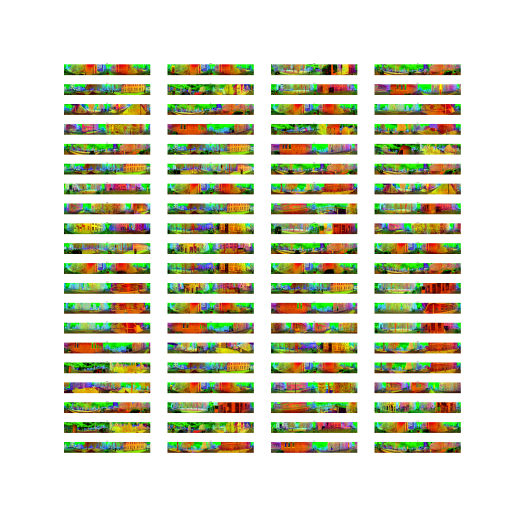
\includegraphics[width=0.16\textwidth]{image_overview/random_all_channels_train_small.png}} 
    \subfigure[]{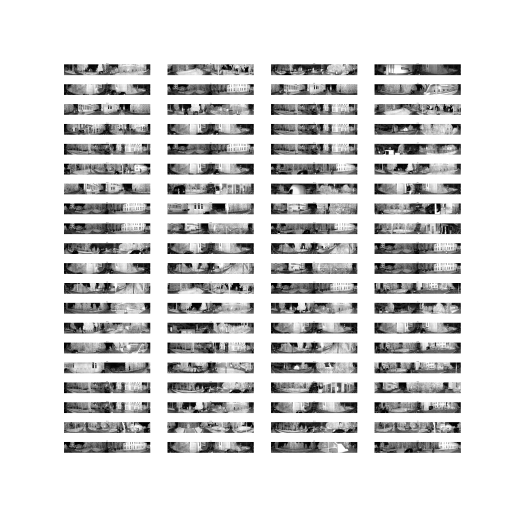
\includegraphics[width=0.16\textwidth]{image_overview/random_channel1_train_small.png}} 
    \subfigure[]{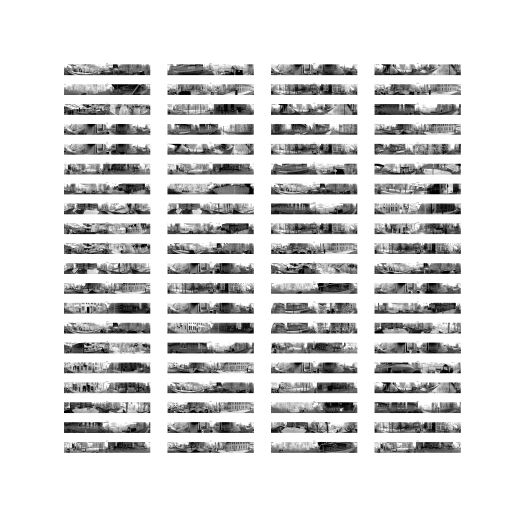
\includegraphics[width=0.16\textwidth]{image_overview/random_channel2_train_small.png}}
    \subfigure[]{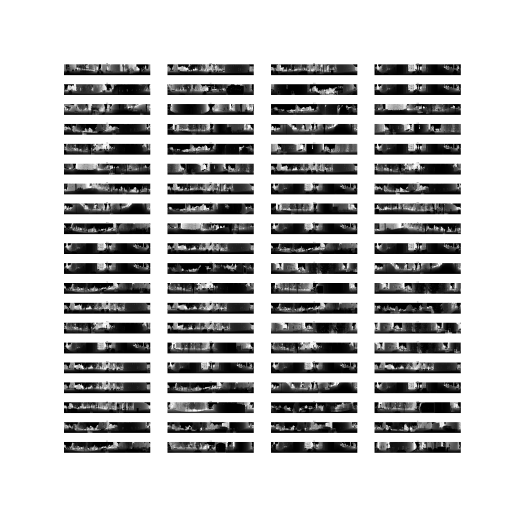
\includegraphics[width=0.16\textwidth]{image_overview/random_channel3_train_small.png}}
    \subfigure[]{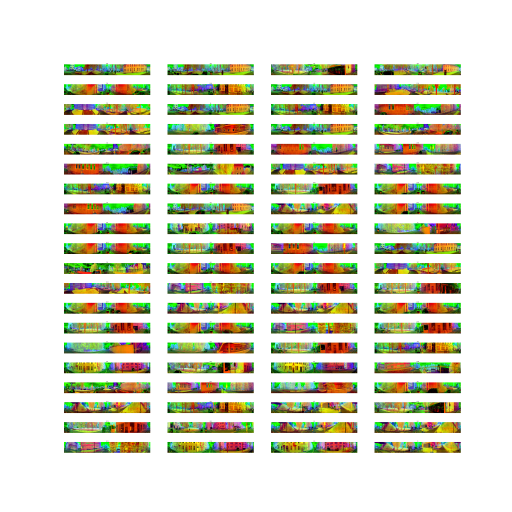
\includegraphics[width=0.16\textwidth]{image_overview/random_car(1)_train_small.png}}
    \subfigure[]{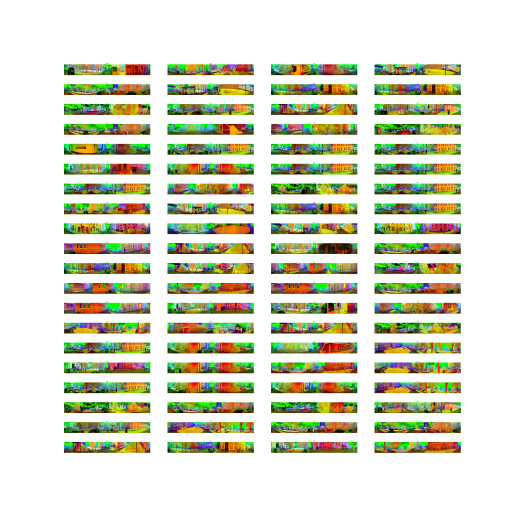
\includegraphics[width=0.16\textwidth]{image_overview/random_person(7)_train_small.png}}
    \caption{Randomly selected images from the original training set showing (a) all three channels combined (b) the first channel (depth) (c) the second channel (ambience) (d) the third channel (intensity) (e) cars (f) persons.}
    \label{fig:overview}
\end{figure}

\subsubsection*{Quantitative analysis}
The prevalent object class in the original training set are cars (52.3\%), followed by persons (26.8\%) and riders of vehicles (8.7\%). This can be seen both from Figure \ref{fig:ratio}, which shows the ratio of labels over the original training set, the updated training set, and the validation set, as well as Figure \ref{fig:occurrence} (a), showing the total occurrence of labels in the training set, the updated training set, and the validation set. While this observation is roughly consistent with the updated extended training set (51.9\% cars, 32.3\% persons, 4.9\% bicycles), the distribution differs significantly from the validation set. Here, the most prevalent object class are persons (66.7\%), followed by cars (25.9\%) and riders (5.7\%). Notably, the validation set does not contain any images with trucks, bicycles, scooters or motorcycles. The existence of riders in the absence of any vehicles that transport riders (bicycles, scooters and motorcycles) in the validation set raises questions, which will be discussed in the following.

Figure \ref{fig:occurrence} offers more insight into correlations of annotated objects, where plot (b) illustrates the occurrence of objects only in images where the label is present, excluding images that do not contain an object of a chosen class. Thereby, grouped occurrences of labels can be detected. For instance, such groupings become visible for bicycles and scooters, but not so much for cars and persons. In other words, if there is a bicycle in an image, it is likely that there are more bicycles in the same image. For persons, Figure \ref{fig:occurrence} indicates that almost all images contain persons, as the value barely fluctuates from subplot \ref{fig:occurrence} (a) to subplot \ref{fig:occurrence} (b).

\begin{figure}[t]
    \centering
    \subfigure[]{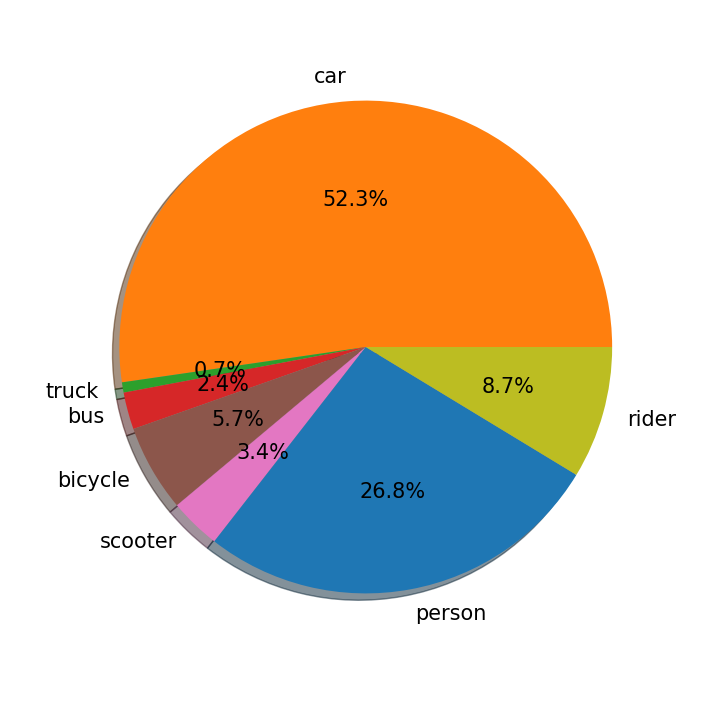
\includegraphics[width=0.32\textwidth]{label_distribution/train/label_ratio_train_cropped.png}}
    \subfigure[]{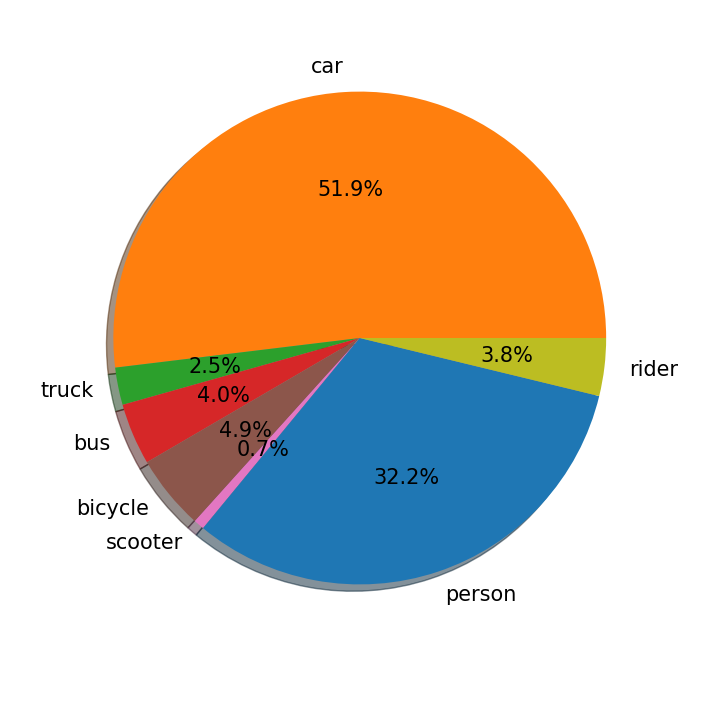
\includegraphics[width=0.32\textwidth]{label_distribution/extended_train/label_ratio_extended_train.png}} 
    \subfigure[]{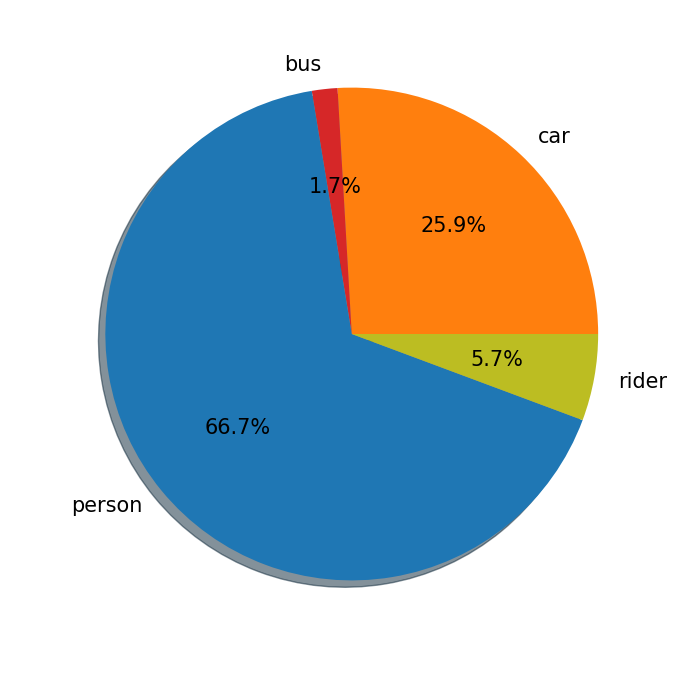
\includegraphics[width=0.32\textwidth]{label_distribution/val/label_ratio_val_cropped.png}} 
    \caption{Label ratios over (a) original training set (b) updated training set (c) validation set.}
    \label{fig:ratio}
\end{figure}

\begin{figure}[t!]
    \centering
    %\subfigure[]{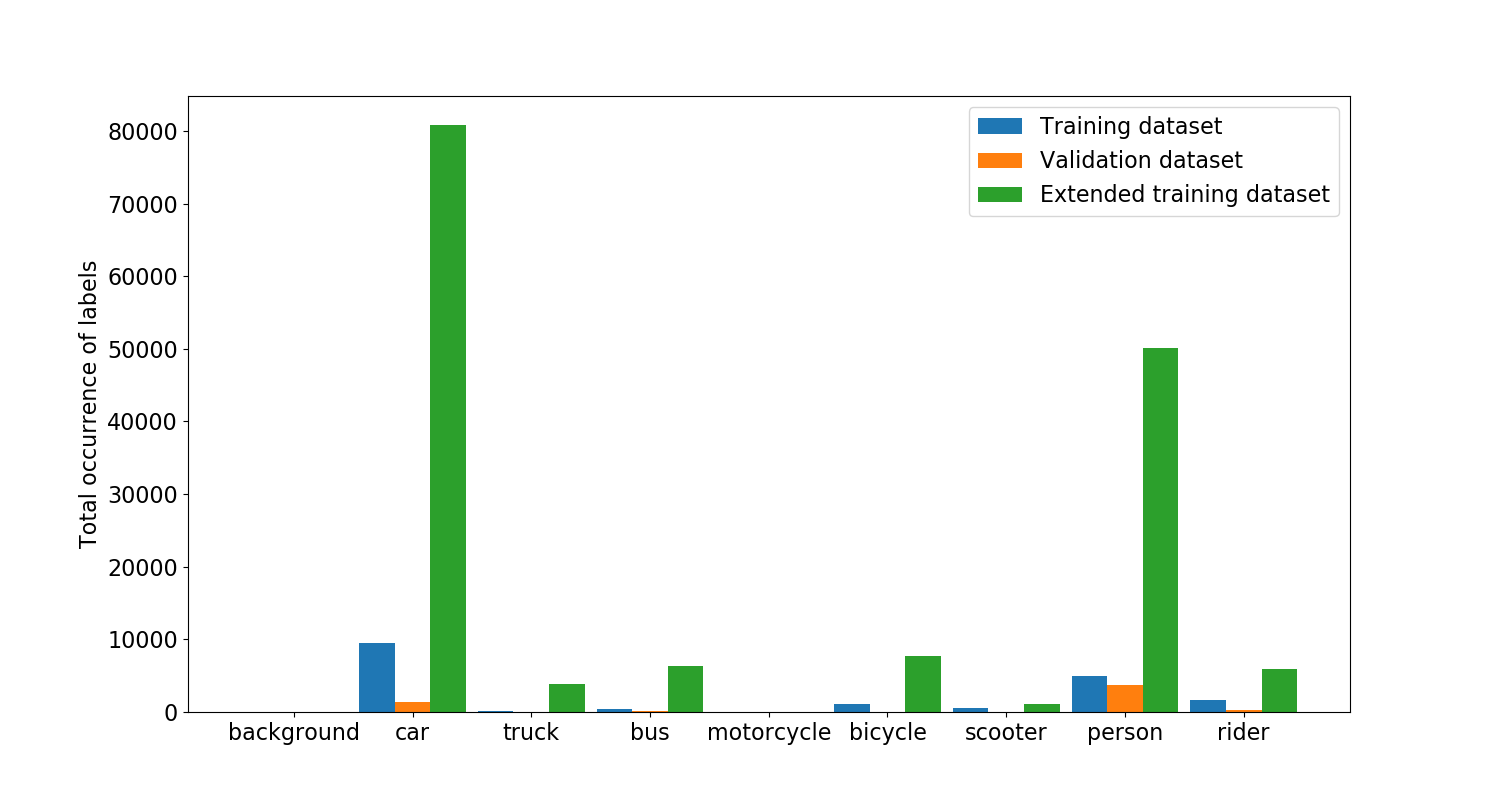
\includegraphics[width=0.49\textwidth]{label_distribution/comparison/total_occurence_comparison.png}}
    %\subfigure[]{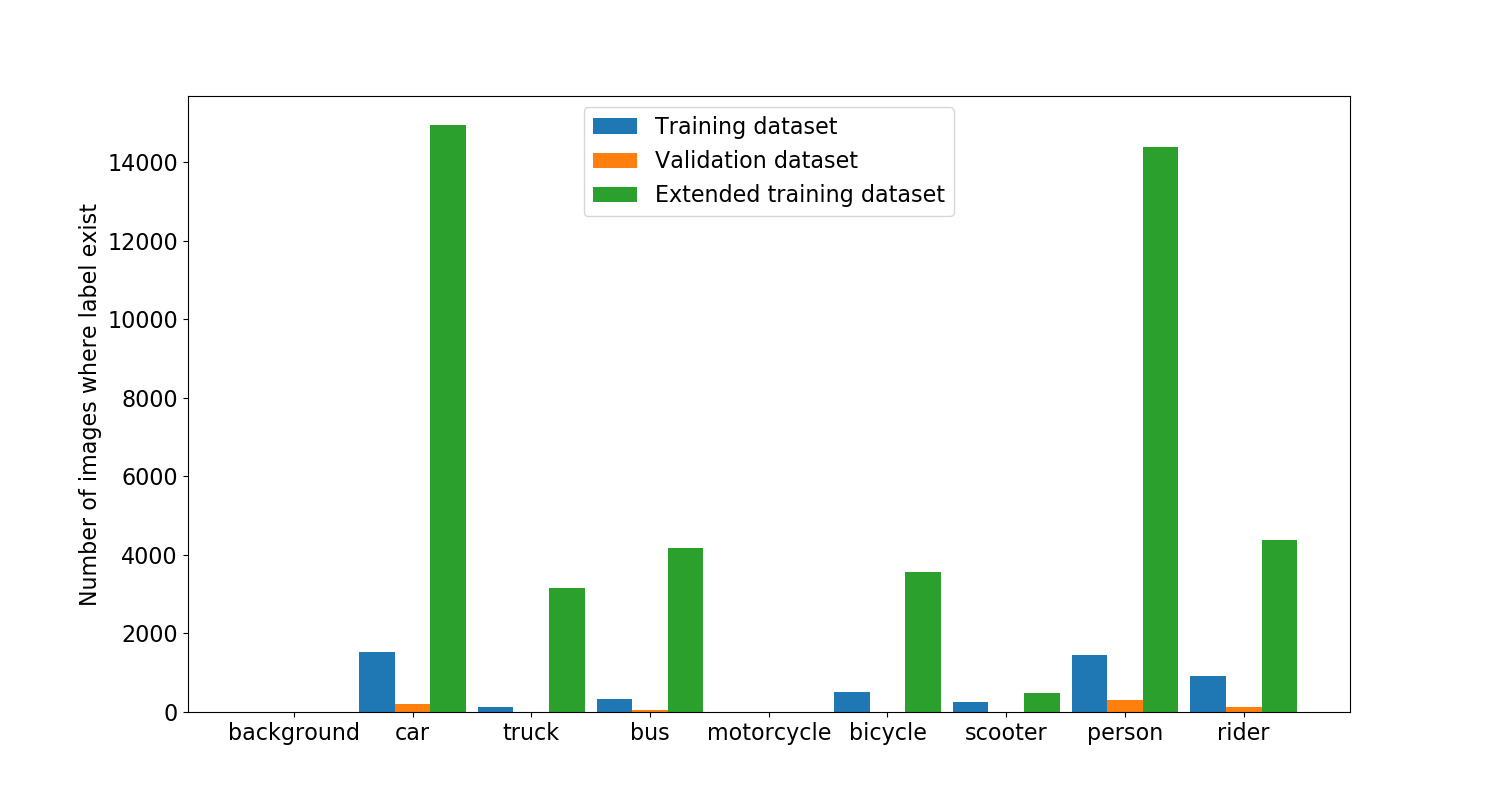
\includegraphics[width=0.49\textwidth]{label_distribution/comparison/number_images_where_label_exist_comparison.png}} 
    \subfigure[]{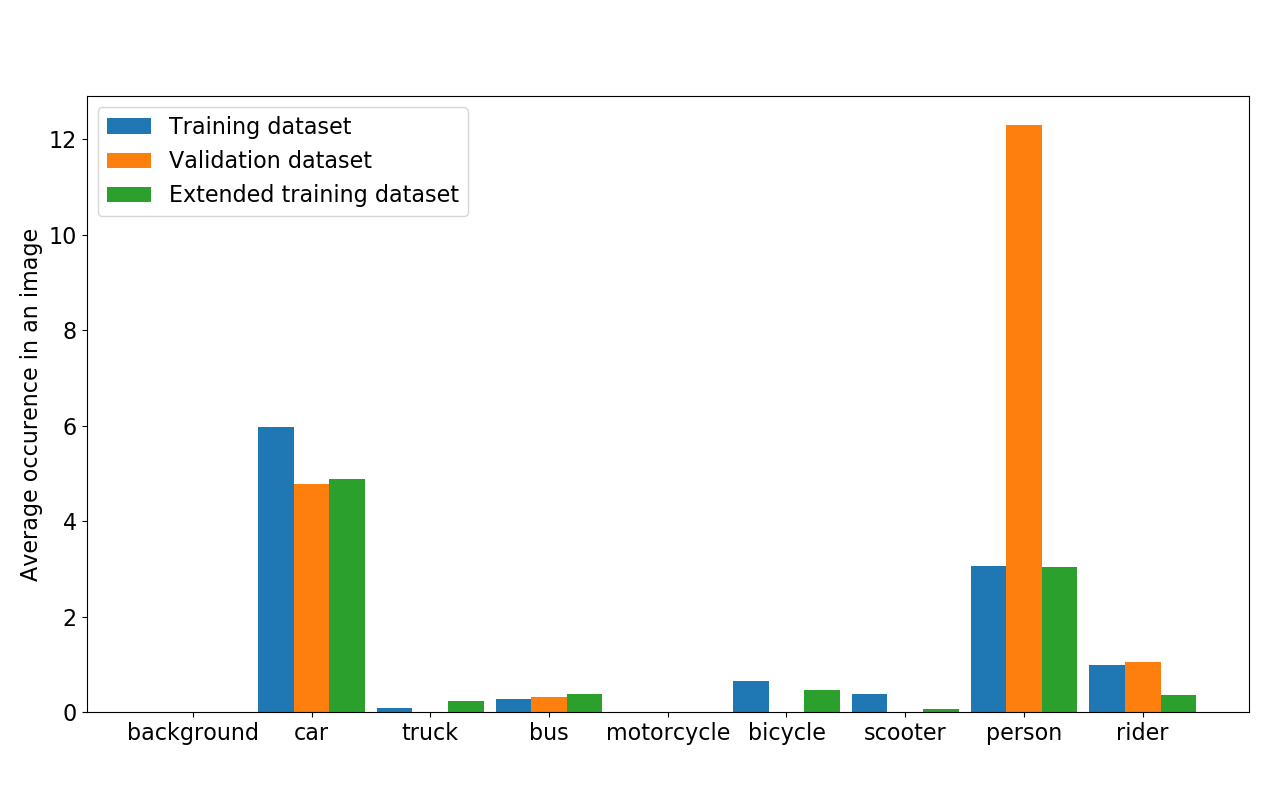
\includegraphics[width=0.49\textwidth]{label_distribution/comparison/avg_occ_comparison.png}} 
    \subfigure[]{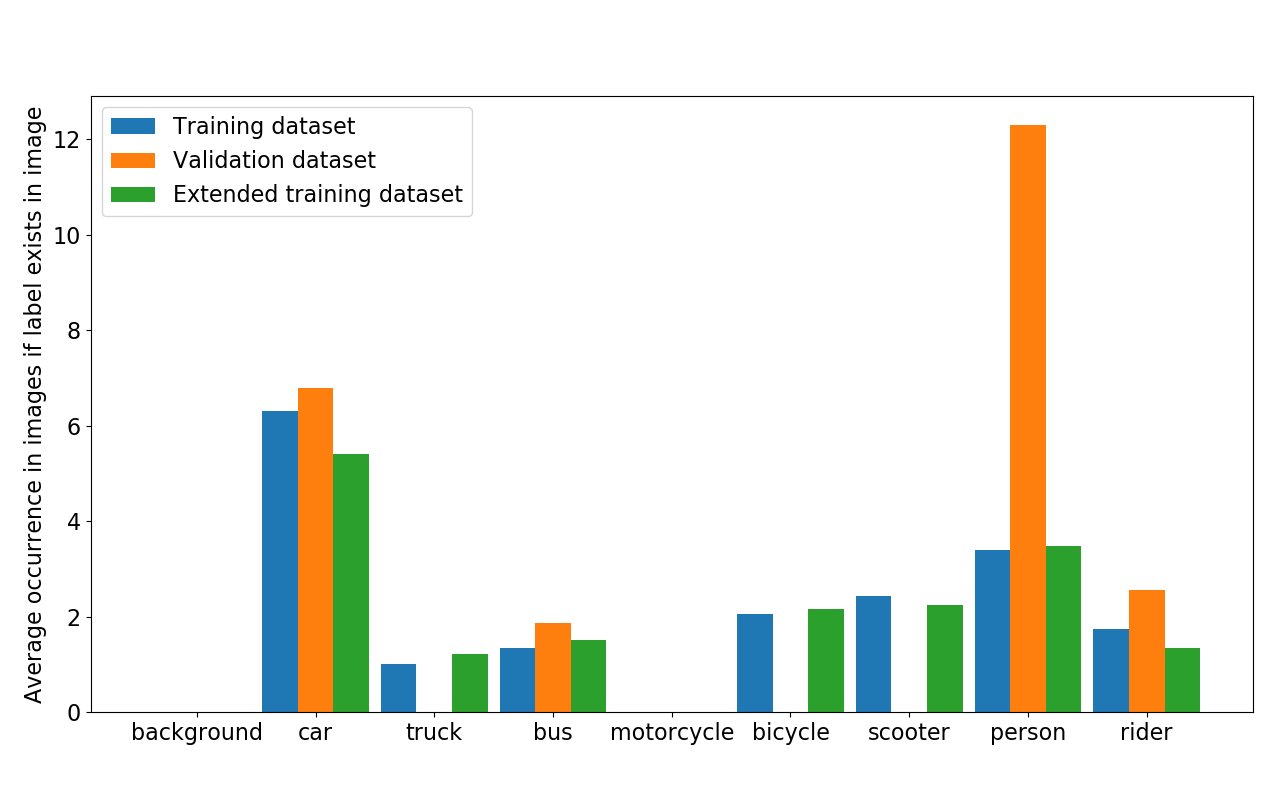
\includegraphics[width=0.49\textwidth]{label_distribution/comparison/avg_occ_if_label_exist_comparison.png}} 
    \caption{Average occurrence of labels (a) over all images (b) in images where the respective label exists.}
    \label{fig:occurrence}
\end{figure}

As a second part of the quantitative analysis, we performed a closer object exploration on the original training dataset and the validation set. This includes the mean area of bounding boxes for each object class as well as histograms of the ratio and size of the bounding boxes over all object classes, which are shown in Figure \ref{fig:objects_expl}. From Figure \ref{fig:objects_expl} (a), it can be seen that trucks and busses have the largest bounding boxes on average, which is consistent with our expectations. Additionally, Figure \ref{fig:objects_expl} (b) shows that there is an overall higher number of smaller bounding boxes in both the training and validation set. The similar distribution allows for the expectation of good validation performance, which shall be examined in the course of this report. Figure \ref{fig:objects_expl} (c) on the other hand shows the frequency of ratios of bounding boxes over both sets. Here, a high number of small ratios, i.e., close to quadratic bounding boxes, can be observed. After a sharp drop, a smaller number of objects has rectangular bounding boxes with a higher ratio of height and width. This leads to the conclusion that there are either somewhat quadratic or somewhat slim bounding boxes, but no continuous transition between the two in both the original training set and the validation set.

Furthermore, \ref{fig:objects_expl} (d) and (e) give the height and width of all bounding boxed for the original training and the validation set as clusters, respectively. Similarly as above, the different distribution of bounding box ratio and size in the original training set and the validation set can be observed. As we have observed from Figure \ref{fig:occurrence}, there is a higher number of persons annotated in the validation set. This is consistent with Figure \ref{fig:objects_expl}, where the bounding boxed for persons, which are small in width but large in height, can be observed distinctly in the cluster. Note that subplots (d) and (e) in Figure \ref{fig:objects_expl} are scaled differently for better visibility. There are however larger bounding boxes in the training set compared to the validation set (consistent with the right tail of subplot (b) of Figure \ref{fig:objects_expl}). As an hypothesis, this could be due to the absence of trucks and busses in the validation set, which are the two largest objects if compared at the same distance. Additionally, there is a high number of cars in the training set, which, if in traffic and captured from a close distance, also have large bounding boxes.

\begin{figure}[t!]
    \centering
    \subfigure[]{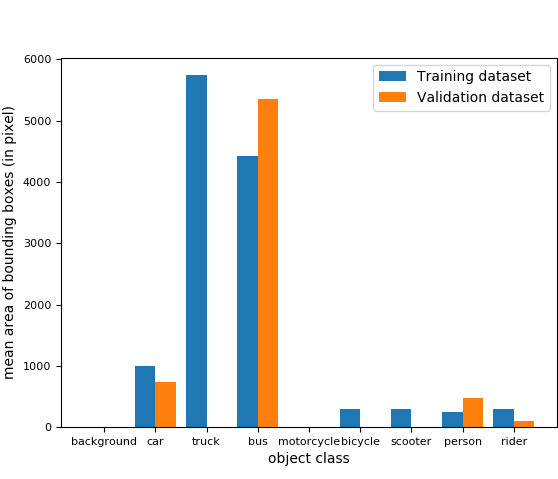
\includegraphics[width=0.32\textwidth]{object_exploration/mean_area_cropped.png}}
    \subfigure[]{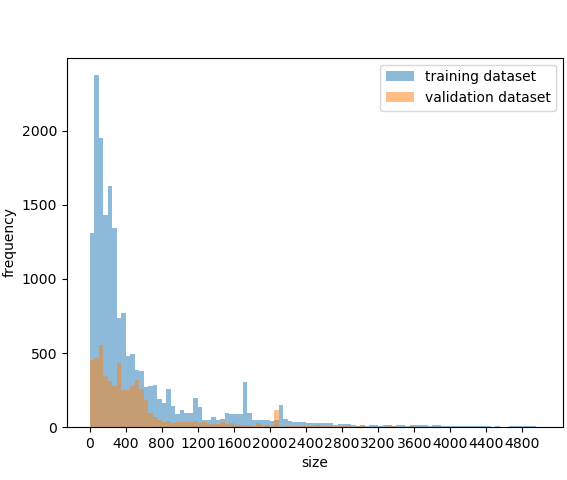
\includegraphics[width=0.32\textwidth]{object_exploration/sizes_cropped.png}}
    \subfigure[]{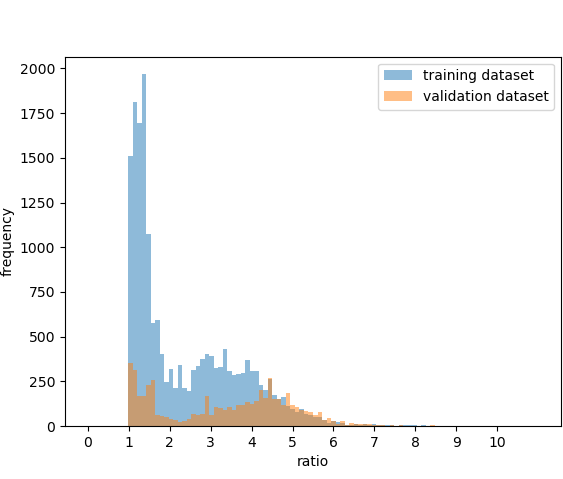
\includegraphics[width=0.32\textwidth]{object_exploration/ratios_cropped.png}}
    \subfigure[]{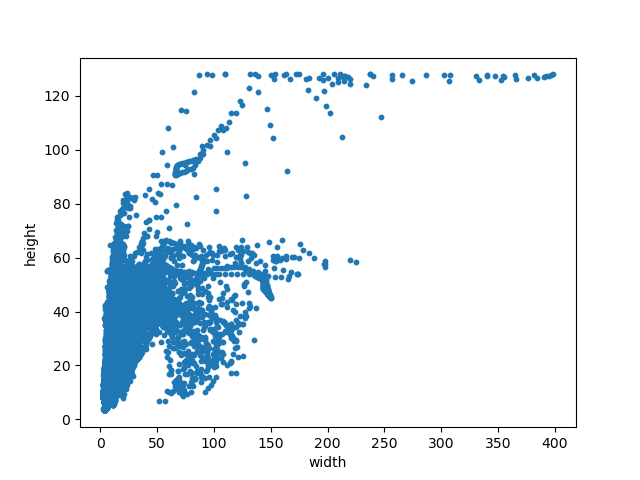
\includegraphics[width=0.4\textwidth]{object_exploration/wh_cluster_train.png}}
    \subfigure[]{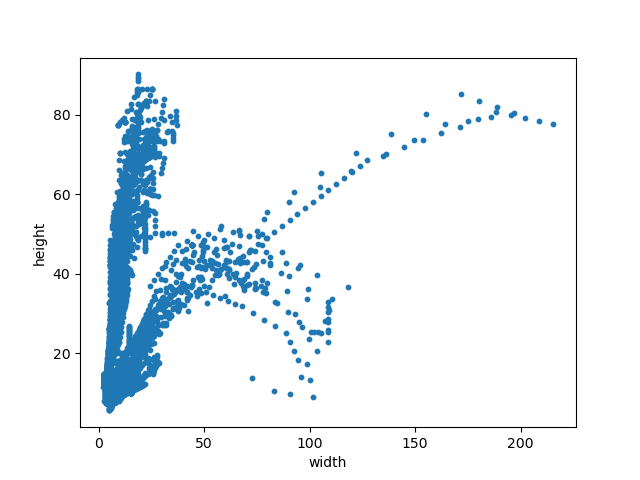
\includegraphics[width=0.4\textwidth]{object_exploration/wh_cluster_val.png}}
    \caption{(a) Mean area of bounding boxes (in pixels) for respective object class (b) histogram of all bounding box sizes (c) histogram of all bounding box ratios (d) cluster of bounding box height and width in the original training set and (e) in the validation set.}
    \label{fig:objects_expl}
\end{figure}

Finally, we investigated some border cases in the dataset to complement the mean observations. Figure \ref{fig:extreme_train} shows the image from the original training set with the maximum (a) and minimum (b) number of annotated objects, the object with the maximum (c) and minimum (d) bounding box ratio and maximum (e) and minimum (f) bounding box size, and the images with the maximum number of cars (g) and persons (h), which are the two most prevalent object categories (see Figure \ref{fig:occurrence}). Figure \ref{fig:extreme_val} presents the same cases for the validation set. Interestingly, the maximum number of objects in an image in the original training set (subplot \ref{fig:extreme_train} (a)) is lower than our expectations, at a total of 22. Contrary to that, the validation set contains an image with 54 annotated objects, all of which are persons. Based on the training data, which only has an image with a maximum number of 9 persons, we expect this to be a challenging validation scenario for the model. Another notable case is subplot \ref{fig:extreme_val} (b), which shows the minimum number of annotated objects in the validation set, which is 4. However, there are a number of unannotated scooters in the middle of the image. The same is true for image \ref{fig:extreme_val} (c) as well as image \ref{fig:extreme_train} (b). Such missing annotations are fatal for the performance in the model if they occur in the training set \cite{xu2019missing} and entail an incorrect accuracy if they appear in the validation set. We have found further images with unannotated objects, among them bikes, busses, and cars, in the original training set. We will follow up on these observations in the following qualitative analysis of the data exploration.

\newpage
\begin{figure}[h!]
    \centering
    \subfigure[]{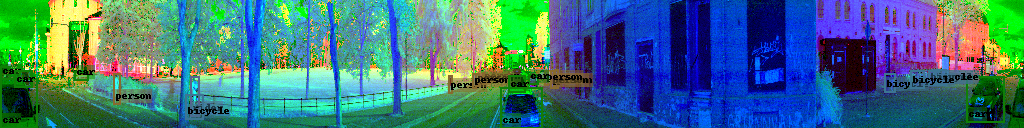
\includegraphics[width=\textwidth]{extreme_cases/train/maximum_num_objects.png}}
    \vspace{-0.15cm}
    \subfigure[]{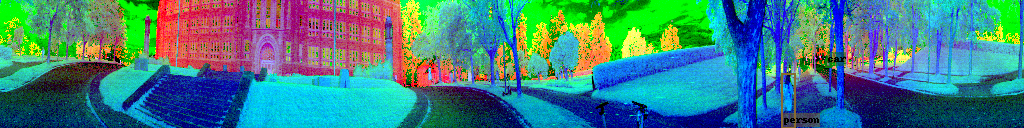
\includegraphics[width=\textwidth]{extreme_cases/train/minimum_num_objects.png}}
    \vspace{-0.15cm}
    \subfigure[]{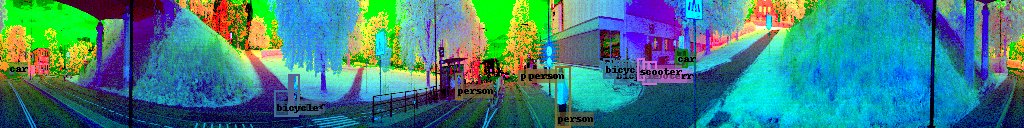
\includegraphics[width=\textwidth]{extreme_cases/train/maximum_ratio.png}}
    \vspace{-0.15cm}
    \subfigure[]{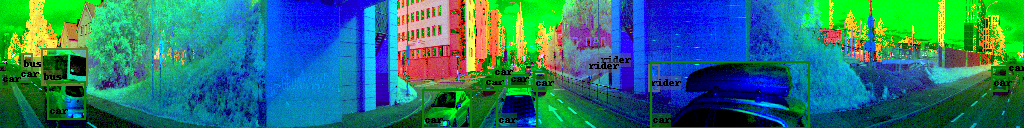
\includegraphics[width=\textwidth]{extreme_cases/train/minimum_ratio.png}}
    \vspace{-0.15cm}
    \subfigure[]{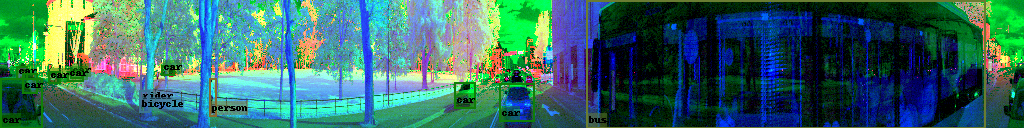
\includegraphics[width=\textwidth]{extreme_cases/train/maximum_size.png}}
    \vspace{-0.15cm}
    \subfigure[]{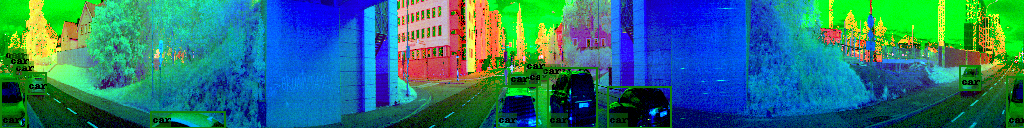
\includegraphics[width=\textwidth]{extreme_cases/train/minimum_size.png}}
    \vspace{-0.15cm}
    \subfigure[]{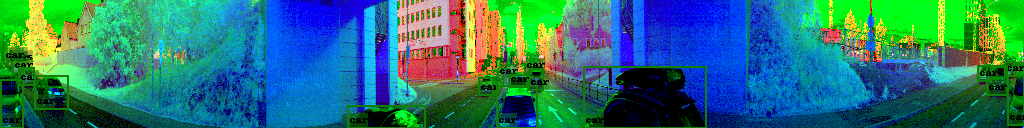
\includegraphics[width=\textwidth]{extreme_cases/train/maximum_num_cars.png}}
    \vspace{-0.1cm}
    \subfigure[]{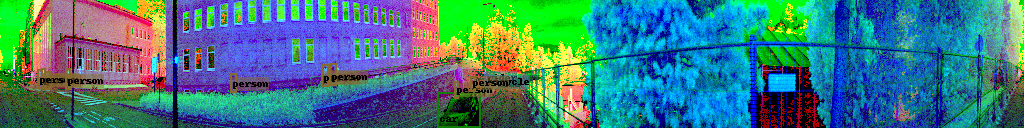
\includegraphics[width=\textwidth]{extreme_cases/train/maximum_num_persons.png}}
    \vspace{-0.49cm}
    \caption{The image from the original training set with (a) the maximum number of annotated objects (22) (b) the minimum number of annotated objects (2) (c) the object with the maximum bounding box ratio (51,046.40 pixels) (d) the object with the minimum bounding box ratio (9.99 pixels) (e) the object with the maximum bounding box size (11.15) (f) the object with the minimum bounding box ratio (1) (g) the maximum number of cars (18) (h) the maximum number of persons (9).}
    \label{fig:extreme_train}
\end{figure}
\newpage

\newpage
\begin{figure}[h!]
    \subfigure[]{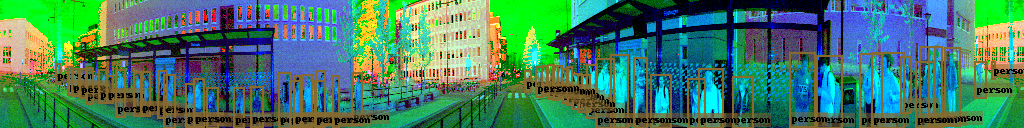
\includegraphics[width=\textwidth]{extreme_cases/val/maximum_num_objects.png}}
    \vspace{-0.15cm}
    \subfigure[]{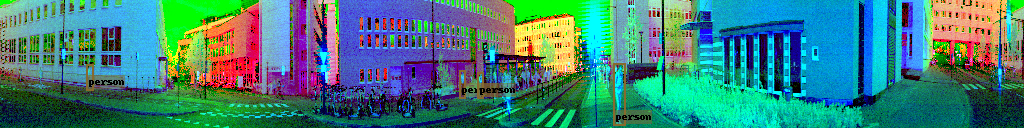
\includegraphics[width=\textwidth]{extreme_cases/val/minimum_num_objects.png}}
    \vspace{-0.15cm}
    \subfigure[]{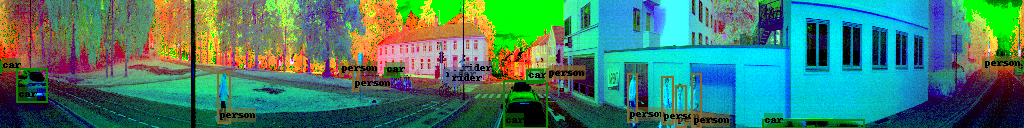
\includegraphics[width=\textwidth]{extreme_cases/val/maximum_ratio.png}}
    \vspace{-0.15cm}
    \subfigure[]{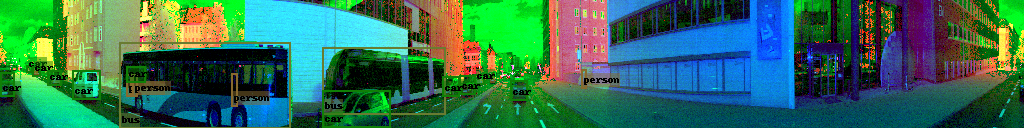
\includegraphics[width=\textwidth]{extreme_cases/val/minimum_ratio.png}}
    \vspace{-0.15cm}
    \subfigure[]{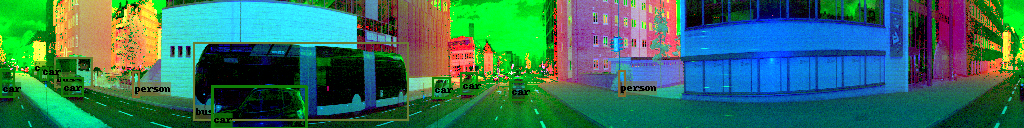
\includegraphics[width=\textwidth]{extreme_cases/val/maximum_size.png}}
    \vspace{-0.15cm}
    \subfigure[]{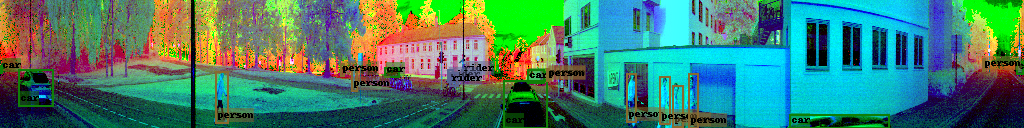
\includegraphics[width=\textwidth]{extreme_cases/val/minimum_size.png}}
    \vspace{-0.15cm}
    \subfigure[]{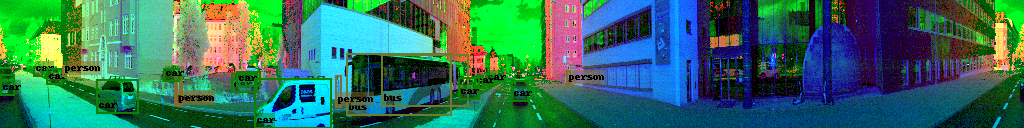
\includegraphics[width=\textwidth]{extreme_cases/val/maximum_num_cars.png}}
    \vspace{-0.1cm}
    \subfigure[]{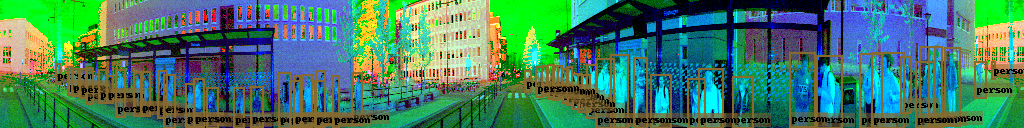
\includegraphics[width=\textwidth]{extreme_cases/val/maximum_num_persons.png}}
    \vspace{-0.49cm}
    \caption{The image from the validation set with (a) the maximum number of annotated objects (54) (b) the minimum number of annotated objects (4) (c) the object with the maximum bounding box ratio (16,760.03 pixels) (d) the object with the minimum bounding box ratio (19.17 pixels) (e) the object with the maximum bounding box size (11.43) (f) the object with the minimum bounding box size (1) (g) the maximum number of cars (12) (h) the maximum number of persons (54).}
    \label{fig:extreme_val}
\end{figure}
\newpage

\subsubsection*{Qualitative analysis}

Going more into depth into the content of the dataset, we oriented to the proposed approach in \cite{Karpathy2019} with the aim of estimating predictions and errors of the model and their reasons. A first questions to be evaluated on the basis of the explored data is whether local or global features are more significant to the outcome of the model performance. In our case, local features in the form of different vehicles and persons in traffic are the most important, while global features such as the brightness, weather or number of vehicles in traffic are of lesser importance. However, of the traffic participants, their global features should be learned by the model in order to classify the desired objects correctly, rather than differentiating within a class based on local features such as the colour of a person's jacket. Additionally, the global context of the objects needs to be correctly recognised by the model, such as the differentiation between a person riding a vehicle, thereby becoming a rider, and a pedestrian.

The variation in the images is generally speaking low. The weather conditions in all captured images are consistent, where there is no precipitation, but snow on the side of the road in the majority of images. The winter conditions also entail that all pedestrians wear similar, winter-appropriate clothing, and that there are no convertibles and no motorcycles (see also Figure \ref{fig:occurrence}). In addition, all data is captured in a tightly limited local area of only a few kilometers within the same city. The volume of traffic is consistently low compared to other areas in the world.

The consistency of the labels in both the training and validation set is critically compromised however. As detailed above and in the video delivered alongside this report, a significant number of labels is either missing or incorrect. This leads to further inconsistencies such as the number of riders compared to the number of vehicles that can transport riders. Therefore, further preprocessing in the form of quality-checking the annotations would be appropriate and expected to improve the model performance across different approaches.

The level of detail in terms of resolution in the evaluated dataset is low. On the one hand, this enables somewhat reasonably efficient training, as the size of the data is limited. On the other hand, the objects to be classified are in many cases hard to detect and correctly bound even for humans, as we experienced during the annotation task of this project at first hand. Therefore, further downsampling of the images is not an option.

As a last point of observation, we conclude that the spatial position of objects in the images matters in the classification task at hand, and should not be average-pooled out. In the context of autonomous driving, which the dataset at hand is arguably relevant for, vehicles and persons should be recognised in any area of the image, as the capturing sensor could for example be looking down onto or up towards a scene of traffic due to hilly roads.

\section*{Task 2: Model Creation}

\subsection*{Task 2.1: Baseline Model}

\begin{table}[t!]
    \small
    \centering
    \begin{tabular}{l|l|c|c|c|c}
        \hline
         Is Output & Layer Type & Number filters & Kernel size & Stride & Padding  \\
         \hline
         & Conv2D & 32 & 3 & 1 & 1 \\
         & ReLU & & & & \\
         & MaxPool2D & & 2 & 2 & 0\\
         & Conv2D & 64 & 3 & 1 & 1\\
         & ReLU & & & & \\
         & Conv2D & 64 & 2 & 1 & 0 \\
         & ReLU & & & &  \\
         & Conv2D & 128 & 2 & 2 & 1\\
         Yes - resolution: $32\times 256$ & ReLU & & & & \\
         \hline
         & ReLU & & & &\\
         & Conv2D & 128 & 3 & 1 & 1\\
         & ReLU & & & & \\
         & Conv2D & 256 & 3 & 2 & 1\\
         Yes - resolution: $16\times 128$ & ReLU & & & & \\
         \hline
         & Conv2D & 256 & 3 & 1 & 1\\
         & ReLU & & & & \\
         & Conv2D & 128 & 3 & 2 & 1\\
         Yes - resolution: $8\times 64$ & ReLU & & & & \\
         \hline
         & ReLU & & & & \\
         & Conv2D & 128 & 3 & 1 & 1\\
         & ReLU & & & & \\
         & Conv2D & 128 & 3 & 2 & 1\\
         Yes - resolution: $4\times 32$ & ReLU & & & & \\
         \hline
         & ReLU & & & & \\
         & Conv2D & 128 & 3 & 1 & 1\\
         & ReLU & & & & \\
         & Conv2D & 64 & 3  & 2 & 1\\
         Yes - resolution: $2\times 16$ & ReLU & & &  & \\
         \hline
         & ReLU & & & & \\
         & Conv2D & 128 & 2 & 2 & 1\\
         & ReLU & & & & \\
         & Conv2D & 64 & 2 & 1 & 0\\
         Yes - resolution: $1\times 8$ & ReLU & & & &\\
         \hline
    \end{tabular}
    \caption{Architecture of baseline model from Task 2.1.}
    \label{tab:baseline}
\end{table}
For this task, we followed all changes given in the task description. The resulting architecture of our baseline model is summarized in Table \ref{tab:baseline}. As recommended, the second max-pool layer of the orginal SSD architecture of assignment 4  was removed and the kernel size of the last two convolutions was set to 2. The baseline model can be found in the configuration file \texttt{configs/tdt4265\_task2-1.py}. It has a total number of 2,750,240 parameters.

The best\footnote{In all quantitative analyses, we give the best mAP@0.5:0.95 that we recorded during the number of epochs trained, which is not always obtained in the last epoch. We implemented this by always saving the current best model.} mAP@0.5:0.95 for the baseline model is 0.037 after 30 epochs, 0.046 after 50 epochs, and 0.054 after 125 epochs. The inference speed is 14.32 frames per second with a total runtime of approximately 6.98 seconds. Plots of the total loss, classification loss, regression loss and mAP can be found in Figure \ref{fig:loss-2-1}. Additionally, we show the AP plots for object classes car and person, which are the two prevalent classes. It can be clearly observed that the AP for cars improves faster and more steadily than for persons, giving a first indication that the classification of the latter is a harder problem for the model. Additionally, we can observe that the AP for class car improves very similarly with the mAP. Knowing that car is the prevalent class in the training set, we can therefore conclude that the training in the baseline model is dominated by this class, and does not perform as well on the remaining classes. This can again be seen when observing the AP for the class person in Figure \ref{fig:loss-2-1} (f).

\begin{figure}[t!]
    \centering
    \subfigure[]{\includesvg[width=0.32\textwidth]{Task2-1/loss_total_loss.svg}}
    \vspace{-0.15cm}
    \subfigure[]{\includesvg[width=0.32\textwidth]{Task2-1/loss_classification_loss.svg}}
    \subfigure[]{\includesvg[width=0.32\textwidth]{Task2-1/loss_regression_loss.svg}}
    \subfigure[]{\includesvg[width=0.32\textwidth]{Task2-1/metrics_mAP.svg}}
    \subfigure[]{\includesvg[width=0.32\textwidth]{Task2-1/metrics_AP_car.svg}}
    \subfigure[]{\includesvg[width=0.32\textwidth]{Task2-1/metrics_AP_person.svg}}
    \vspace{-0.4cm}
    \caption{(a) Total loss (b) classification loss (c) regression loss (d) mAP (e) AP for class car (f) AP for class person for baseline model of Task 2.1 trained for 125 epochs.}
    \label{fig:loss-2-1}
\end{figure}


\subsection*{Task 2.2: Data Augmentation}
In terms of data augmentation, we experimented with six different transformations. In addition to the two already implemented, horizontal flip and random crop, we implemented augmentations through random Gaussian blur, random translation, random dropout and random noise. Visualisations of all six augmentations are shown in Figure \ref{fig:data_augment}, and details can be found in the config files \texttt{configs/tdt4265\_task2-2\_hori\_flip.py}, \texttt{[...]\_crop.py}, \texttt{[...]\_gaussian\_blur.py},\\ \texttt{[...]\_translation.py}, \texttt{[...]\_dropout.py} and \texttt{[...]\_noise.py}.


\begin{figure}[h!]
    \subfigure[]{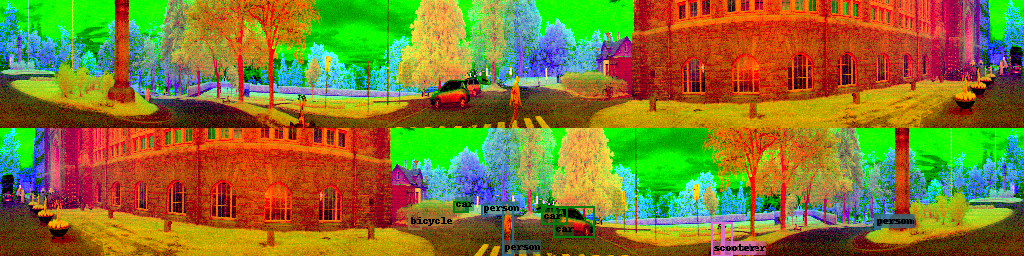
\includegraphics[width=0.49\textwidth]{Task2-2/horizontal_flip/image_9.png}}
    \vspace{-0.15cm}
    \subfigure[]{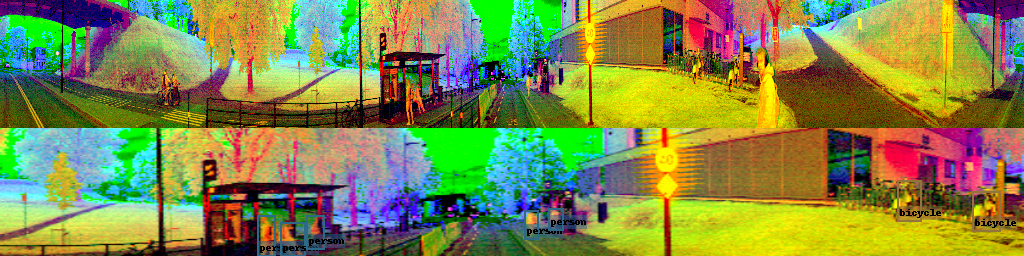
\includegraphics[width=0.49\textwidth]{Task2-2/crop/image_275.png}}
    \vspace{-0.15cm}
    \subfigure[]{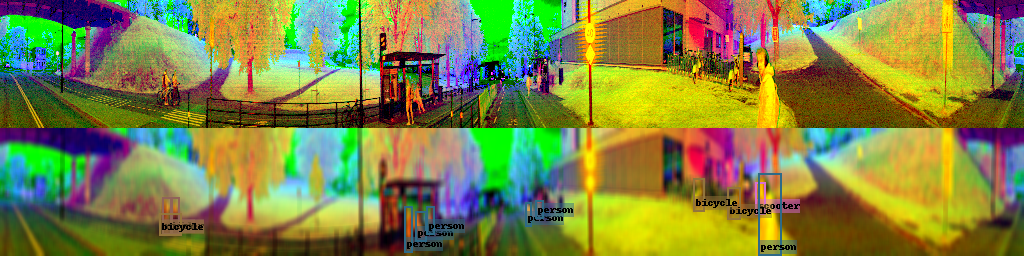
\includegraphics[width=0.49\textwidth]{Task2-2/gaussian_blur/image_275.png}}
    \vspace{-0.15cm}
    \subfigure[]{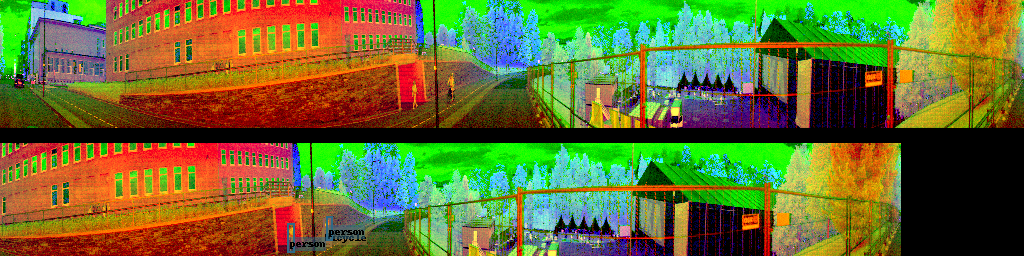
\includegraphics[width=0.49\textwidth]{Task2-2/translation/image_175.png}}
    \vspace{-0.15cm}
    \subfigure[]{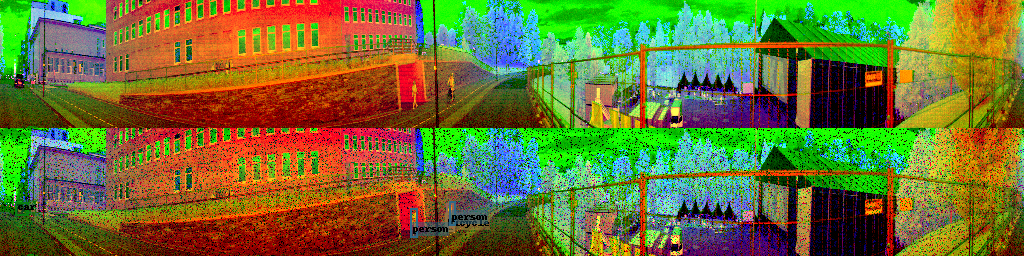
\includegraphics[width=0.49\textwidth]{Task2-2/dropout/image_175.png}}
    \vspace{-0.15cm}
    \hspace{0.2cm}\subfigure[]{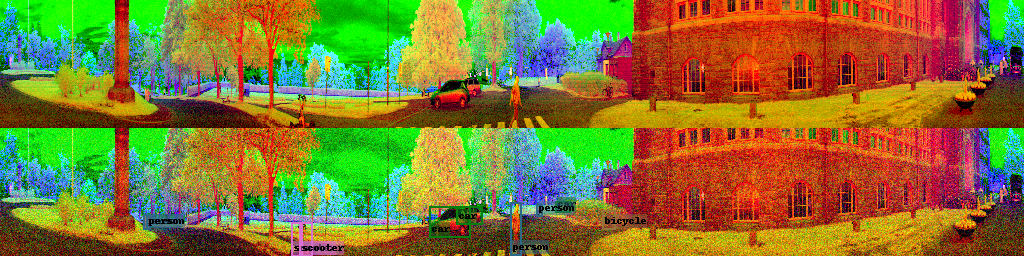
\includegraphics[width=0.49\textwidth]{Task2-2/noise/image_9.png}}
    \vspace{-0.15cm}
    \caption{Data augmentation by means of (a) random horizontal flip (b) random crop (c) random Gaussian blur (d) random translation (e) random dropout (f) random noise. The top image of each subplot is the original image, the bottom image the augmented image.}
    \label{fig:data_augment}
\end{figure}

\subsubsection*{Quantitative Analysis}
Plots of losses for the baseline model in combination with the different augmentations are shown in Figure \ref{fig:loss-2-2-better}, which shows all augmentation approaches that improve the performance compared to the baseline system, and Figure \ref{fig:loss-2-2-worse}, showing all approaches with worse performance. Overall, each augmentation is evaluated individually with the baseline model, i.e., augmentations are not stacked upon each other. The best mAP@0.5:0.95 after 125 epochs is 0.057 with random horizontal flip, 0.062 with random crop, 0.059 with random Gaussian blur, 0.062 with random translation, 0.055 with random dropout and 0.050 with random noise.

Despite training for an increased number of epochs, none of the data augmentation methods improve the mAP significantly compared to the baseline model of Task 2.1. The best empirical argument can be made for random translation and random crop, which both achieve the highest mAP, and arguably provide similar transformations on the training data. This observation supports our assumption that learning objects independent of their spatial position is important to the performance of the model. Furthermore, with the translation of the image, the model learns features of categories with less context, since for example the pavement under a person could be shifted out of the image. While the training dataset provides this, the augmentation by cropping and translating adds to the model experiencing such situations. Contrary to that, adding noise or dropping out pixels are not helpful to the model. We presume that the resolution of the images is already a lower bound for the model, and adding further disturbance to the information presented is too much of a challenge. Horizontal flip and Gaussian blur barely change the performance of the model.

The inference speed and the number of parameters do not change under data augmentation.

\begin{figure}[t!]
    \centering
    \subfigure[]{\includesvg[width=0.32\textwidth]{Task2-2/better/loss_total_loss4.svg}}
    \vspace{-0.15cm}
    \subfigure[]{\includesvg[width=0.32\textwidth]{Task2-2/better/loss_classification_loss4.svg}}
    \subfigure[]{\includesvg[width=0.32\textwidth]{Task2-2/better/loss_regression_loss4.svg}}
    \subfigure[]{\includesvg[width=0.32\textwidth]{Task2-2/better/metrics_mAP4.svg}}
    \subfigure[]{\includesvg[width=0.32\textwidth]{Task2-2/better/metrics_mAP@0.5_4.svg}}
    \subfigure[]{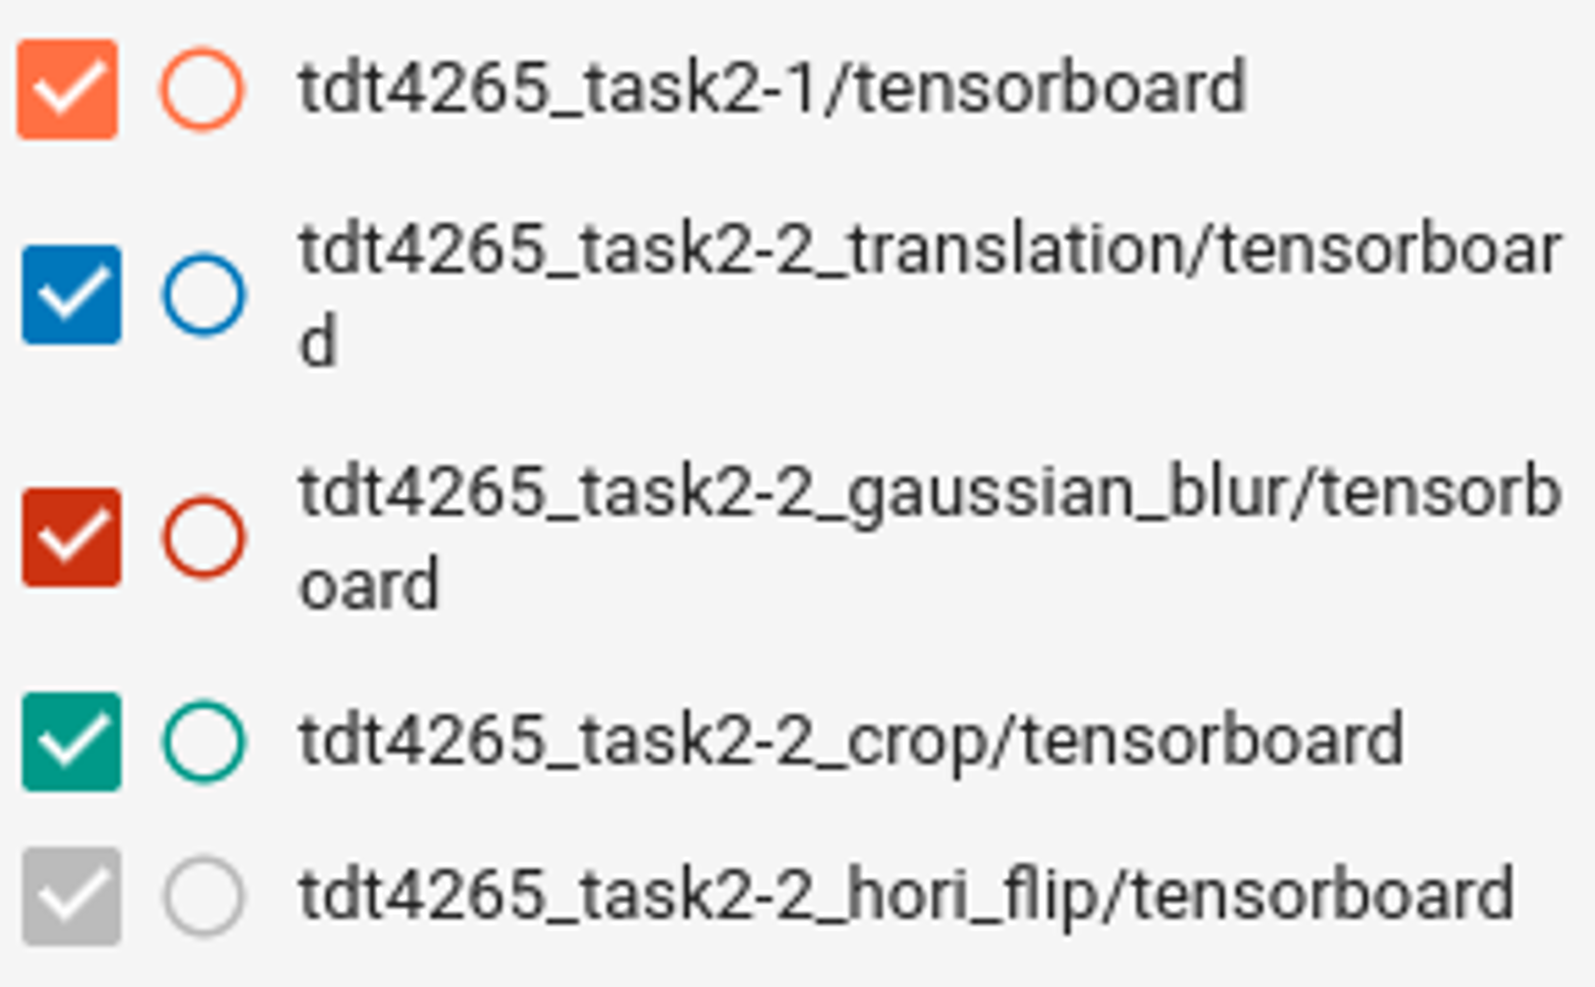
\includegraphics[width=0.32\textwidth]{Task2-2/legend-2-2-better1.png}}
    \vspace{-0.3cm}
    \caption{(a) Total loss (b) classification loss (c) regression loss (d) mAP (e) mAP@0.5 (f) legend for data augmentation of Task 2.2 trained for 125 epochs, performing better than the baseline model from Task 2.1 (in terms of mAP).}
    \label{fig:loss-2-2-better}
\end{figure}

\begin{figure}[t!]
    \centering
    \subfigure[]{\includesvg[width=0.32\textwidth]{Task2-2/worse/loss_total_loss2.svg}}
    \vspace{-0.15cm}
    \subfigure[]{\includesvg[width=0.32\textwidth]{Task2-2/worse/loss_classification_loss2.svg}}
    \subfigure[]{\includesvg[width=0.32\textwidth]{Task2-2/worse/loss_regression_loss2.svg}}
    \subfigure[]{\includesvg[width=0.32\textwidth]{Task2-2/worse/metrics_mAP2.svg}}
    \subfigure[]{\includesvg[width=0.32\textwidth]{Task2-2/worse/metrics_mAP@0.5.svg}}
    \subfigure[]{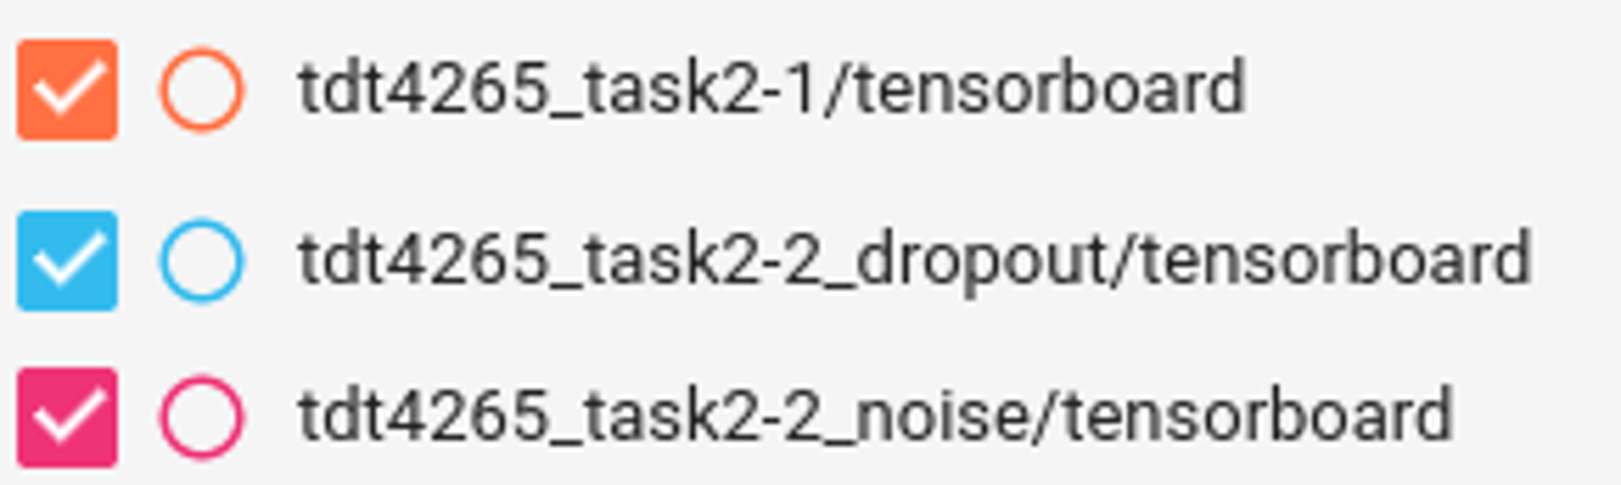
\includegraphics[width=0.32\textwidth]{Task2-2/legend-2-2-worse.png}}
    \vspace{-0.3cm}
    \caption{(a) Total loss (b) classification loss (c) regression loss (d) mAP (e) mAP@0.5 (f) legend for data augmentation of Task 2.2 trained for 125 epochs, performing worse than the baseline model from Task 2.1 (in terms of mAP).}
    \label{fig:loss-2-2-worse}
\end{figure}

\subsubsection*{Runtime Performance}
Loading the images from the original training set without any augmentations comes at a speed of approximately 104.83 images per seconds. In comparison, data loading with random crop achieves 120.73, random dropout 99.51, random blur 107.48, horizontal flip 101.15, random Gaussian noise 105.43, and finally random translation only 35.16 images per seconds, respectively.

\subsubsection*{Combining the Data Augmentation}
Finally, we combined the four data augmentations that yielded a better performance than the baseline model individually. A plot of the mAP using the combined augmentations can be found in Figure \ref{fig:data_augment_comparison} (a). The mAP@0.5:0.95 comes out at 0.54 after training for 167 epochs. While this does not give an improvement to the precision achieved with the Task 2.1 baseline model, its benefits will become evident once the model becomes more complex in Task 2.3.

The runtime for dataloading in this case dropped down to 48.82 images per second. Due to the high cost of data loading, and at the recommendation of one of the instructors, we decided to go forward with the following tasks without using data augmentation on the original training set. Only at the end of Task 2.3, we add the combined data augmentation back in (see Figure \ref{fig:data_augment_comparison} (b)) to evaluate its effect on the more complex model. 

\subsection*{Task 2.3: Implementing RetinaNet}

\subsubsection*{Feature Pyramid Network}
Coming from the Task 2.1 baseline mode, we replaced the first four layers of the model by the first four layers of the  pretrained ResNet34 model from the torchVision model zoo \cite{pytorchModelZoo}. For the fifth and sixth feature extraction layer, we used a sequence of a convolutional layer with 512 channels, kernel size 3, stride 1, padding 1 followed by ReLU activation function, a MaxPool2D layer with kernel size 2 and stride 2, a second convolutional layer with 256 channels, kernel size 3, stride 1 and padding 1, and a ReLU activation to conclude the feature extraction layer, respectively. Finally, we built the Feature Pyramid Network (FPN) on top of the six feature extraction layers as described in \cite{lin2017feature} with channel size 256 and the same number of aspect ratios for each layer, as anticipation for later use of deeper classification and regression heads and for better comparability and a more meaningful analysis.

Replacing the backbone of the baseline model with a FPN yielded a best mAP@0.5:0.95 after 100 epochs of 0.056. Details can be found in the config file \texttt{configs/tdt4265\_task2-3\_fpn}.  The implementation of the FPN can be found in the file \texttt{modeling/backbones/resnet34\_fpn.py}.  A plot of losses is given in Figure \ref{fig:loss-2-3}, where the FPN model is shown in dark blue. The model has a total number of 35,382,204 parameters and an inference speed of approximately 8.34 frames per seconds, with a total runtime of 11.10 seconds, which is faster than the Task 2.1 baseline model.

Applying the Resnet34 with a FPN on top only helps in detecting more medium sized objects (see Figure \ref{fig:loss-2-3} (h)). The detection of both large and small objects is not improved (\ref{fig:loss-2-3} (g) and (i), respectively). This is a surprising result, since the objective of the FPN is mainly to provide semantically rich feature maps for smaller object sizes. Nevertheless, the mAP@0.5:0.95 increases by 0.2\% with 25 epochs less training time compared to the baseline model in Task 2.1.

\subsubsection*{Focal Loss}
As described in the task, we replaced the loss function with Focal loss \cite{lin2017focal} with the recommendations made in the task description. This includes implementing Focal loss on top of the softmax cross-entropy loss, for which we applied one-hot encoding of the given target labels. Details can be found in the file \texttt{ssd/modeling/focal\_loss.py}. For this task, we chose $\gamma = 2$ as recommended in \cite{lin2017focal} and set $\alpha = 0.01$ for the background class as indicated in the task. 

By these changes, the performance of best mAP@0.5:0.95 at 0.056 after 100 epochs is maintained in comparison to the FPN without Focal loss. The config file is \texttt{configs/tdt4265\_task2-3\_focal}. A plot of losses is given in Figure \ref{fig:loss-2-3}, where the model with Focal loss is shown in light blue. The inference speed and the total number of parameters remain the same as in the previous step.

Focal loss adds a factor to the cross entropy loss function, which reduces the loss especially for well-classified examples, but also suppresses the loss function overall \cite{lin2017focal}. This property can be observed in the classification loss: Focal loss seems to decrease the classification loss compared to the previous model. As seen in Figure \ref{fig:loss-2-3}, the classification loss approaches 0 much faster than the previous models. Another reason for the low classification loss might also be the low alpha value for the background class, which could lead to lower classification loss than with the previous hard negative mining in the previous loss function. 


\begin{figure}[t!]
    \centering
    \subfigure[]{\includesvg[width=0.32\textwidth]{Task2-3/loss_total_loss3.svg}}
    \subfigure[]{\includesvg[width=0.32\textwidth]{Task2-3/loss_classification_loss3.svg}}
    \subfigure[]{\includesvg[width=0.32\textwidth]{Task2-3/loss_regression_loss3.svg}}
    \subfigure[]{\includesvg[width=0.32\textwidth]{Task2-3/metrics_mAP3.svg}}
    \subfigure[]{\includesvg[width=0.32\textwidth]{Task2-3/metrics_mAP@0.5_3.svg}}
    \subfigure[]{\includesvg[width=0.32\textwidth]{Task2-3/metrics_mAP_small3.svg}}
    \subfigure[]{\includesvg[width=0.32\textwidth]{Task2-3/metrics_mAP_medium3.svg}}
    \subfigure[]{\includesvg[width=0.32\textwidth]{Task2-3/metrics_mAP_large3.svg}}
    \subfigure[]{\includesvg[width=0.32\textwidth]{Task2-3/metrics_AP_car3.svg}}
    \subfigure[]{\includesvg[width=0.32\textwidth]{Task2-3/metrics_AP_person3.svg}}
    \subfigure[]{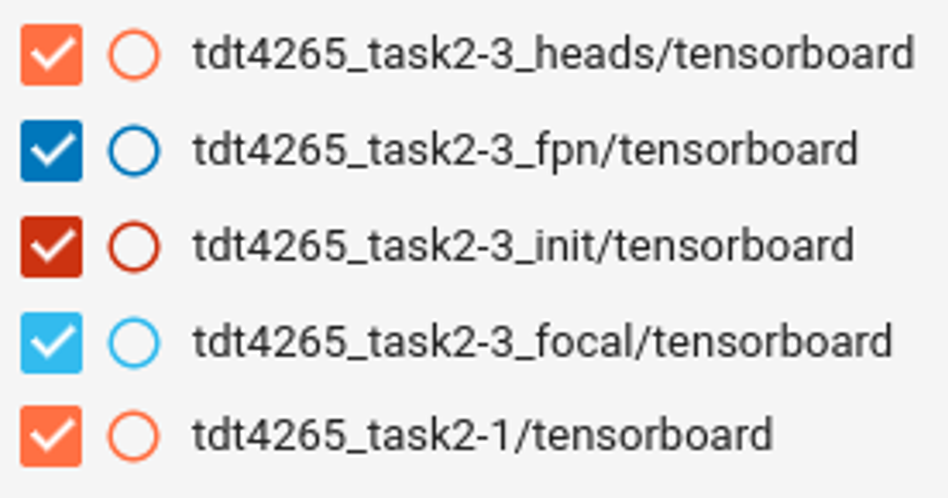
\includegraphics[width=0.32\textwidth]{Task2-3/legend-2-3.png}}
    \caption{(a) Total loss (b) classification loss (c) regression loss (d) mAP (e) mAP@0.5 (f) mAP for small objects (g) mAP for medium objects (h) mAP for large objects (i) AP for object class car (j) AP for object class person (k) legend for the iterations in Task 2.3 trained for 100 epochs. The baseline system of Task 2.1 is represented by the orange plot, which can be differentiated from the plot for the adapted classification and regression heads as it was trained for a longer number of 125 epochs (and performs consistently worse).}
    \label{fig:loss-2-3}
\end{figure}

\subsubsection*{Deeper Classification and Regression Output Heads}
 We implemented deeper regression and classification heads following the architecture used in \cite{lin2017focal}. Details can be found in the file \texttt{ssd/modeling/RetinaDeep.py}. In our implementation, all feature map extractions share the same parameters, and in both heads, we used four convolutional layers with channel size 256, kernel size 3, stride 1 and padding 1 followed by ReLU activation each. The last layer of the classification head is now a convolutional layer with channel size n\_boxes $\times$ num\_classes, and the last layer of the regression head is a convolutional layer with channel size n\_boxes $\times$ 4.
 
Replacing the single-layer regression and classification output heads with deeper convolutional nets comes with an observable improvement in performance, with the best mAP@0.5:0.95 with in 100 epochs being 0.070. The config file is \texttt{configs/tdt4265\_task2-3\_heads}. The model has a total number of 39,203,894 parameters and an inference speed of 3.03 frames per second, for a total of 33.03 seconds. A plot of losses is given in Figure \ref{fig:loss-2-3}, where the model with deeper classification output heads is shown in orange.

Deeper classification and regression heads provide the ability to learn more complex patterns from the extracted feature maps in order to recognise objects and adapt the anchor boxes to the object. This property can be easily observed in the Figure \ref{fig:loss-2-3}, which clearly shows the large improvements in terms of mAP@0.5:0.95 in each object sizes and overall. On the other side, the larger amount of parameters in the classification and regression heads also introduce a higher loss as can be seen in the loss functions (see Figure \ref{fig:loss-2-3} (a) - (c)).

\subsubsection*{Initialisation of Bias}

As a last step in Task 2.3, the initialisation was be implemented, which follows the recommendations in the paper \cite{lin2017focal}. More precisely, we initialized all bias parameter in both the regression and the classification head to 0 but the bias for the background class of the last layer of the classification head, which corresponds to the recommendation in the task. All weights in both the regression and the classification head were initialized to a Gaussian distribution with mean of 0 and standard deviation of 0.1. The initialization should prevent the model from experiencing a high loss value from the large amount of background anchors. We did not observe any high values in the first iterations after introducing focal loss and contrarily saw a low loss value after a few iterations. Thus, we do not see any improvements with the initialization as implemented in the paper. Nevertheless, we observed that the loss function decreases with the initialization, which is the expected behaviour. The model with the initialization even results in a slightly worse mAP@0.5:0.95 of 0.069 after training for 100 epochs.

Further details of our implementation can be found in the file \texttt{ssd/modeling/retina\_deep\_init.py} and the config file \texttt{configs/tdt4265\_task2-3\_init.py}. A plot of losses is given in Figure \ref{fig:loss-2-3}, where the model with improved initialisation of the bias is shown in red.


\subsubsection*{Adding Data Augmentation Back In}

Initially, we trained the models in Task 2.3 without any augmentations to yield a better comparison between the introduced features and to save time during data loading. After implementing all required features from Task 2.3, we reintroduced several data augmentations we had previously evaluated on the Task 2.1 model in order to prevent the model from the apparent overfitting. More precisely, we applied the augmentations random crop, random horizontal flip, random translation and random Gaussian blur to the Task 2.3 model, as those were the ones with the best performance improvements on the Task 2.1 baseline model. Figure \ref{fig:data_augment_comparison} shows the effect of the described data augmentation on (a) the Task 2.1 baseline model in comparison to (b) the Task 2.3 model in terms of mAP. While its benefits were not yet visible in the Task 2.1 model, enlarging the training set by augmentations evidently helps to prevent the Task 2.3 model from overfitting.

\begin{figure}[b!]
    \centering
    \subfigure[]{\includesvg[width=0.4\textwidth]{Task2-2/final/metrics_mAP7.svg}}
    \subfigure[]{\includesvg[width=0.4\textwidth]{Task2-3/metrics_mAP_with_augmentations.svg}}
    \caption{(a) Task 2.1 baseline model with (blue) and without (orange) data augmentation (b) Task 2.3 model with (pink) and without (red) data augmentation as detailed in Task 2.2.}
    \label{fig:data_augment_comparison}
\end{figure}


\newpage
\subsection*{Task 2.4: Using the Exploration Knowledge}

\subsubsection*{Alpha}
In order to counter the harsh imbalance in the data set as seen in the data exploration, we followed the approach to modify the alpha values in the focal loss function according to the prevalence of the classes in the training data set. For this, we assigned specific values for $\alpha$ detailed in Table \ref{tab:alpha}.

\begin{table}[h!]
    \centering
    \begin{tabular}{c|c|c}
    Object class & Label ratio (training) & assigned $\alpha$\\
    \hline
    car & 52.3\% & 1\\
    person & 26.8\% & 1.95\\
    rider & 8.7\% & 6.00 \\
    bicycle & 5.7\% & 9.10 \\
    scooter & 3.4\% & 15.4 \\
    bus & 2.4\% & 21.80 \\
    truck & 0.7\% & 75.00 \\
    motorcycle & 0.0\% & 0 \\
    \end{tabular}
    \caption{New values for $\alpha$ derived from the data exploration analysis.}
    \label{tab:alpha}
\end{table}

In this way, we expected a more balanced result for the different classes, since mistakes in regressing and classifying less frequently represented examples lead to a higher loss than the more prevalent examples, like the cars. Thus, there's a higher incentive for the model to focus on the rare objects.

As we can see in \ref{fig:loss-2-4-mAP}, the overall mAP improves significantly. Furthermore, one can see an increase in the detection of smaller objects, which might be the result of focusing on smaller objects than the most prevalent class car.

\subsubsection*{Gamma}

Focal loss has another parameter to adapt to the dataset: $\gamma$. Since the model focuses on the classes, which are easy to classify, predominantly the car, we expected that increasing the $\gamma$ should result in a more balanced result, since the incentive for the model increases to avoid classification and regression mistakes in classes harder to classify, e.g. a person (which is in a lot of cases hard to recognize even for a human being).

As we can see in \ref{fig:loss-2-4-mAP}, the overall mAP increases slightly. In \ref{fig:loss-2-4-sml}, one can see that the model better classifies small objects, since smaller objects are generally harder to detect than larger.

\subsubsection*{Anchors}

The size and the ratio of the anchors of a object detection model should be as close to the data set as possible, in order to make regression and classification efficient for the model.

First, we decided to cluster the sizes of the along the size of the objects in order to determine groups of ground truth boxes which are in similar size. These clusters of boxes are then again clustered along the with and height in order to determine the boxes in the data set, which are in similar ratio. In each size group of the boxes three different ratios are determined.

For the clustering we used the k-means implementation of the scikit package \cite{scikit-learn}.

\begin{figure}[h!]
    \centering
    \subfigure[]{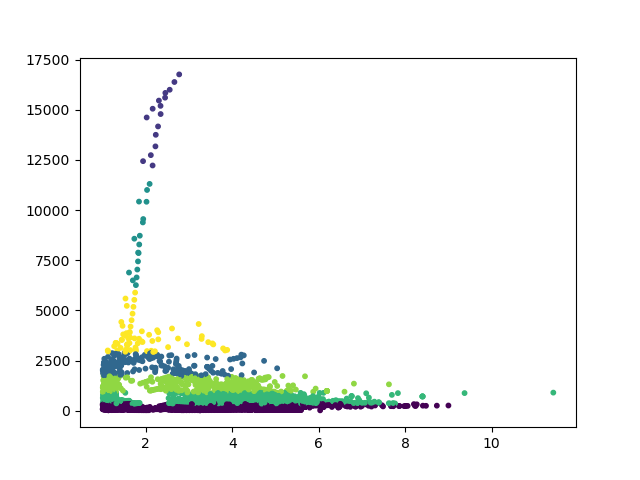
\includegraphics[width=0.32\textwidth]{Task2-4/Anchors/cluster.png}}
    \subfigure[]{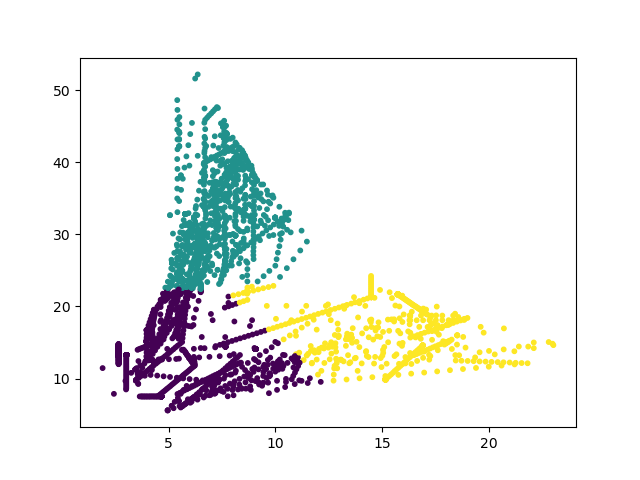
\includegraphics[width=0.32\textwidth]{Task2-4/Anchors/cluster_0.png}}
    \vspace{-0.15cm}
    \subfigure[]{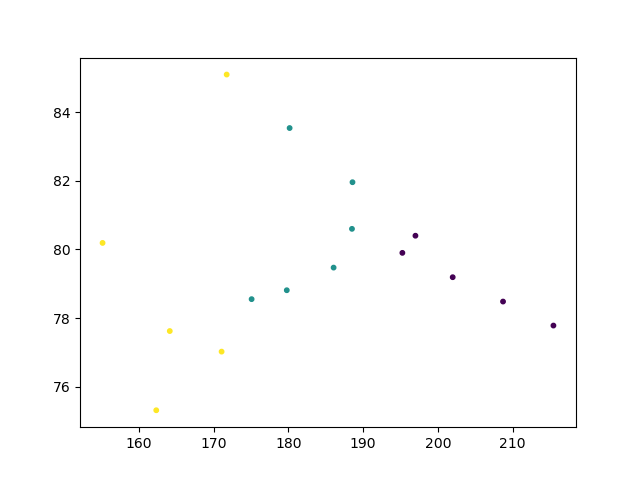
\includegraphics[width=0.32\textwidth]{Task2-4/Anchors/cluster_1.png}}
    \subfigure[]{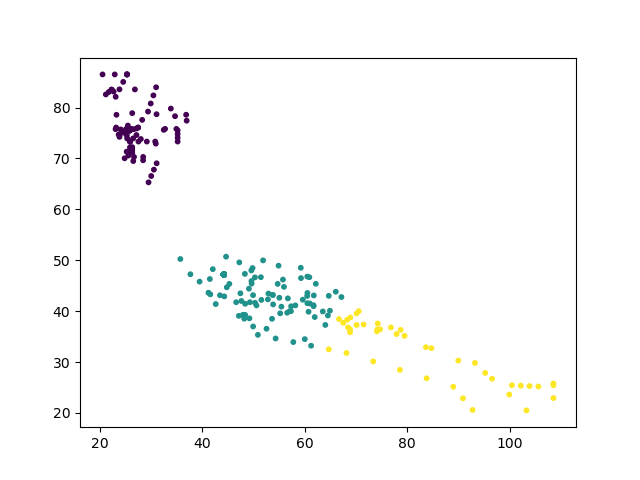
\includegraphics[width=0.32\textwidth]{Task2-4/Anchors/cluster_2.png}}
    \vspace{-0.15cm}
    \subfigure[]{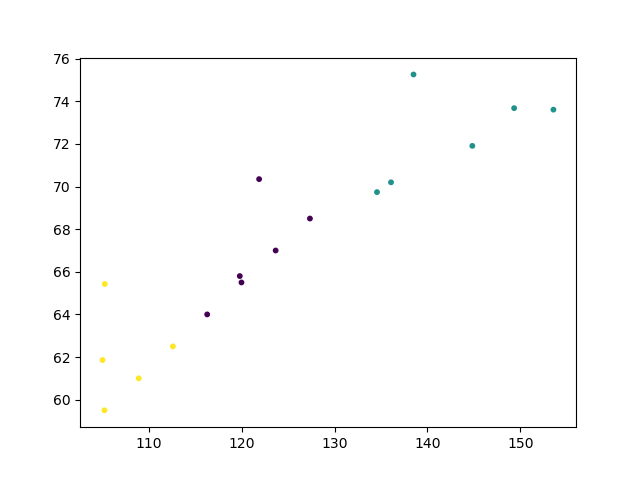
\includegraphics[width=0.32\textwidth]{Task2-4/Anchors/cluster_3.png}}
    \subfigure[]{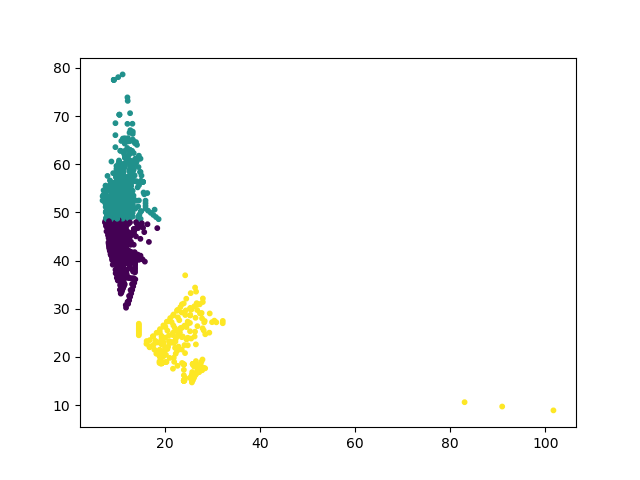
\includegraphics[width=0.32\textwidth]{Task2-4/Anchors/cluster_4.png}}
    \vspace{-0.15cm}
    \subfigure[]{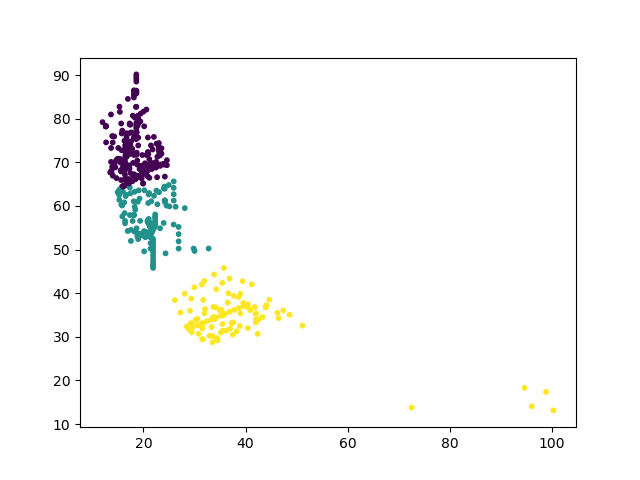
\includegraphics[width=0.32\textwidth]{Task2-4/Anchors/cluster_5.png}}
    \vspace{-0.15cm}
    \caption{\textcolor{red}{(a)  Clustering the sizes of the boxes in the validation set (b-f) clustering the ratios of the groups of boxes.}}
    \label{fig:clustering}
\end{figure}

As we can see in \ref{fig:loss-2-4-mAP}, we can see a small decrease in the mAP, but looking at \ref{fig:loss-2-4-sml} we see that there is a significant increase in the mAP for the small object sizes, since the anchor boxes are optimized. The small decrease of the overall mAP can be traced back to the general difficulty of classifying smaller objects, since there are less features prevalent.

\subsubsection*{Feature Map}

Until now, the model scales down the actual image to a feature map of [32, 128] in the first feature map extraction, by a factor of 4. We considered, that this might be a too large factor for the smaller objects in the image to be recognized by the anchor boxes. Therefore, we tried out to change the size of the first feature map in order to see the difference. Yet, we were aware that introducing a bigger feature map introduces an extreme inference overhead, which might yield a worse performance.

\subsubsection*{Regression and Classification Heads}

Until now, the model uses one head for all the feature maps regarding classification and regression. In the data exploration step we discovered, that there are classes which are predominantly emerging in smaller sizes, e.g. a person. Cars on the other hand are double the size on average. Thus, we considered to split the regression and the classification head into two, so that the model can learn the smaller objects independently from the larger objects. In order to be able to train within the memory limit of our resources, we reduced the depth of the heads each.

As seen in \ref{fig:loss-2-4-mAP}, the overall mAP stays almost the same. Yet, looking at \ref{fig:loss-2-4-sml}, we see that small objects are better detected by the model. The detection of the medium sized objects is worse. This could be traced back to the fact that the medium sized objects are split along the two heads, which are then overall trained worse each.


\subsubsection*{Final}
We concluded that the following adaptions are worth following: Alpha, Gamma, Anchors, Heads.

As a final step, we also introduced the Adam optimizer \cite{kingma2014adam}. Adam uses the Adaptive Gradient Algorithm, which applies different learning rates for different parameters. In this way, the optimizer makes it possible to learn sparse features more efficiently. As seen in Task 1.1, the images in the dataset consist of a low resolution and predominantly smaller objects. Thus, the Adam optimizer introduces a good mechanism to make the model learn these sparse features more efficiently.

Furthermore, we applied the augmentations from Task 2.2.

In Figure \ref{fig:loss-2-4}, one can clearly see the significant improvement in overall mAP, as well as in the detection for each object size compared to the model from Task 2.2. The mAP@0.5:0.95 increases to 0.092 overall. The amount of parameters is 39590904. The runtime analysis results in 22.77s total runtime and 4.39 FPS.

\begin{figure}[t!]
    \centering
    \subfigure[]{\includesvg[width=0.32\textwidth]{Task2-4/Alpha/metrics_mAP9.svg}}
    \subfigure[]{\includesvg[width=0.32\textwidth]{Task2-4/Anchors/metrics_mAP11.svg}}
    \subfigure[]{\includesvg[width=0.32\textwidth]{Task2-4/Gamma/metrics_mAP12.svg}}
    \subfigure[]{\includesvg[width=0.32\textwidth]{Task2-4/Heads/metrics_mAP13.svg}}
    \subfigure[]{\includesvg[width=0.32\textwidth]{Task2-4/Feature-Map/metrics_mAP14.svg}} 
    \caption{mAP for (a) Alpha (b) Anchors (c) Gamma (d) Heads (e) Feature Map, where the Task 2.3 model is shown in red.}
    \label{fig:loss-2-4-mAP}
\end{figure}


\newpage
\begin{figure}[t!]
    \centering
    \subfigure[]{\includesvg[width=0.32\textwidth]{Task2-4/Final/loss_total_loss10.svg}}
    \subfigure[]{\includesvg[width=0.32\textwidth]{Task2-4/Final/loss_classification_loss10.svg}}
    \subfigure[]{\includesvg[width=0.32\textwidth]{Task2-4/Final/loss_regression_loss10.svg}}
    \subfigure[]{\includesvg[width=0.32\textwidth]{Task2-4/Final/metrics_mAP10_10.svg}}
    \subfigure[]{\includesvg[width=0.32\textwidth]{Task2-4/Final/metrics_mAP_small10.svg}}
    \subfigure[]{\includesvg[width=0.32\textwidth]{Task2-4/Final/metrics_mAP_medium10.svg}}
    \subfigure[]{\includesvg[width=0.32\textwidth]{Task2-4/Final/metrics_mAP_large10.svg}}
    \subfigure[]{\includesvg[width=0.32\textwidth]{Task2-4/Final/metrics_AP_car(1)10.svg}}
    \subfigure[]{\includesvg[width=0.32\textwidth]{Task2-4/Final/metrics_AP_person10.svg}}
    \caption{(a) Total loss (b) classification loss (c) regression loss (d) mAP (e) mAP for small objects (f) mAP for medium objects (g) mAP for large objects (h) AP for object class car (i) AP for object class person for Task 2.4 model using the exploration knowledge.}
    \label{fig:loss-2-4}
\end{figure}
\newpage

\subsection*{Task 2.5: Extending the Dataset}

For training the extended data set we used the best model yet, which is the final model developed in Task 2.4. The mAP@0.5:0.95 increases to 0.195. Runtime analysis yields a total runtime of 22.73s and 4.4 FPS. The total parameter stays the same.

The importance of a larger dataset can be directly seen by the severe improvements in mAP. The difference in mAP between the same model trained with a small dataset and the large dataset is 10\% and thus more than twice as precise (in terms of the mAP metric). This can be traced back to the fact, that a larger dataset provides a wider representation of the domain.

\begin{figure}[t!]
    \centering
    \subfigure[]{\includesvg[width=0.32\textwidth]{Task2-5/loss_total_loss6.svg}}
    \vspace{-0.15cm}
    \subfigure[]{\includesvg[width=0.32\textwidth]{Task2-5/loss_classification_loss6.svg}}
    \subfigure[]{\includesvg[width=0.32\textwidth]{Task2-5/loss_regression_loss6.svg}}
    \subfigure[]{\includesvg[width=0.32\textwidth]{Task2-5/metrics_mAP6.svg}}
    \caption{(a) Total loss (b) classification loss (c) regression loss (d) mAP@0.5:0.95 (e) mAP}
    \label{fig:loss-2-5}
\end{figure}


\newpage
\section*{Task 3}

\subsection*{Task 3.1}
Delivered in Task 2 and 4.

\subsection*{Task 3.2}
Select three 3 of the most influential modeling decisions throughout the project and present a qualitative analysis. The qualitative analysis should highlight key aspects of your model and should be supported by qualitative
examples.

\subsubsection*{Feature Pyramid Network}
Applying the pretrained Resnet34 model with a FPN on top is one of the decisive modelling decisions.

The pretrained network approaches the maximum mAP much faster than the training the model from scratch \ref{fig:loss-2-3}. This results in less computing time and less resource demand. This could already be a decisive decision, since GPU resources are often the dominant factor in developing an object detection model.

With the pretrained resnet model and the FPN on top, the model increases the mAP especially in detecting medium sized objects. The mAP for medium sized objects is increasing by a significant 2\%. This is visible looking at the inference results in \ref{fig:comparison1}. Medium sized objects like the person on the left or the rider on the hill are not recognized by the baseline model, the model with FPN on the other side detects more smaller sized objects. This is crucial for a model in this domain, since the ability to detect smaller object increases the safety of the car.

\begin{figure}[t!]
    \centering
    \subfigure[]{\includegraphics[width=0.5\textwidth]{Task3-2/image_2_baseline.png}}
    \subfigure[]{\includegraphics[width=0.5\textwidth]{Task3-2/image_2_FPN.png}}
    \label{fig:comparison1}
\end{figure}

The model is mainly limited by the small training dataset, since the overfitting kicks in quite early. This behaviour is also due the fact, that there was initially no augmentations applied. But while the baseline model still approaches higher mAPs, the new model does not seem to increase after around 500 iterations.

The model decision improves the ability of detecting smaller objects, since the FPN introduces semantically rich feature maps with a high resolution.

The paper \cite{efficientdet} states several advanced alternatives to the Feature Pyramid networks: PANet, NAS-FPN and the proposed BiFPN. The BiFPN was applied in Task 4, but yielded no better precision. Thus, the FPN might be the better alternative in this case.

\subsubsection*{Deeper classification and regression heads}

Deeper classification and regression heads enable the model to learn a wider range of patterns in the features from the feature extractor, which result in better regression and classification results, which can be observed in \ref{fig:loss-2-3}. The model especially improves in the ability to detect smaller objects, having an almost twice as good mAP on small objects then all the models before. One can see that especially in \ref{fig:comparison2} on the rightmost side. The person far away is not recognized by the previous FPN model, but almost perfectly detected by the model with deeper heads.

\begin{figure}[t!]
    \centering
    \subfigure[]{\includegraphics[width=0.5\textwidth]{Task3-2/image_276_fpn.png}}
    \subfigure[]{\includegraphics[width=0.5\textwidth]{Task3-2/image_276_head.png}}
    \label{fig:comparison2}
\end{figure}

The model is able to learn the sparse features in the feature map corresponding to a person far away. This is decisive for a car, since recognizing danger far away can increase the chance of a proper reaction in time.

The model is limited by the amount of additional parameters. The complex model yields a long inference time and a lower FPS. Instead of around 8 frames per second, the model can only process around 3 frames per second. Thus, the model could be too slow to be working in the domain of autonomous cars, since the reaction time to incoming images could be too slow to be considered safe.

Alternatively, the deeper heads could be replaced by smaller heads, which would lead to a much faster inference time. This approach would reduce the complexity of the model and thus the ability of detecting objects with sparse features. In this case, a compromise has to be found between the expressiveness and the speed of the model.


\subsubsection*{Data augmentation}

Data augmentation is crucial in a small data set as the original one. Artificially extending the dataset prevent the model from early overfitting and thus lead to a higher mAP. This can be observed in Task 2.3, where we trained the complex model with and without augmentations \ref{fig:data_augment_comparison}. The final model of Task 2.3 starts to overfit at around 1500 iterations, while model with augmentations improves in mAP until 5000 iterations to a final mAP of 0.09 compared to 0.063 in the same model trained without augmentations. 

The reason for the improvement of 2.7\% is mainly the fact that the artificially increased dataset avoids that the model remembers the features in the small number of images instead of learning the represented features.

The method is mostly limited by the fact that the number augmentations, which can be applied to an image is limited. Artificially increasing the dataset is only going well until a certain limit. If the augmented images are too far away from the images they represent, the model could learn wrong features.

Alternatively, the model could be trained on a larger data set, as it happened in Task 2.5. Yet, enlarging the data set is often not possible or expensive.


\subsection*{Task 3.3}
What are the weaknesses of the approach selected in the project if you were to deliver this to a customer?

The small validation set is definitely a weakness when it comes to estimating the performance of the model. In an idle world, the model would be tested on another representative independent data set. This stops the development of the model from fitting the modeling decisions to the small data set, which might not even be representative at all.

Furthermore, we observed a lot of wrong labels in the training, as well as in the validation data set. This could mean, that the model is either learning wrong objects, or the metrics, e.g. the mAP, are less representative. In the case of autonomous cars, this represents a severe safety issue.

The inference time could be a problem in the domain of autonomous cars. Processing 4 frames per second might be too slow to follow the safety requirements.

Another problem could be the relatively large size of the model in terms of storage. Systems in autonomous cars have limited storage resources and the size of around 3GB could be too large.


\section*{Task 4}

\subsection*{Task 4.1: Implementing BiFPN}

For the implementation of BiFPN, we used the available implementation of \cite{efficientdet}. The model corresponds to the model developed in Task 2.3 with small adaptions. For example, the last two feature extractors are replaced by only one convolutional layer each (kernel size 3, stride 2, padding 1). Furthermore we adapted the existing implementation of the BiFPN to process 4 layers instead of 3 layers from the feature extractor in order to get 6 feature maps from the backbone. We used the Bi-FPN implementation with 64 channels and 3 blocks.

The runtime of the BiFPN model is Total 12.31s with a FPS value of 8.12. The best best mAP@0.5:0.95 is at 0.072 after 3750 iterations (75 epochs). The number of parameters is 22511987.




\subsection*{Task 4.2: Explaining the Model with CAM}

For the CAM we used the grad\_cam package as recommended by the task \cite{gradcam}. We had to introduce following adaptations to get it run within our implementation. At first, we had to implement a custom reshape function, which reshapes the activation to a specific target size. Second, the implementation in the package expects a dictionary as results from the model, which is contrary to the current implementation, where we return a tuple for the results. Thus, we wrapped the model in a custom wrapper, which returns the results in a dictionary instead of a tuple. It can be found in \texttt{ssd/modeling/retina\_wrap.py}. Furthermore, we decided to use the available script from the repository to implement the CAM visualisation and compare it to the actual image. We used \texttt{performance\_assessment/save\_comparison\_images.py}. The implementation can be found in \texttt{performance\_assessment/class\_activation.py}. The script automatically loads random images from the data set and applies the cam activation, which is then saved to \texttt{performance\_assessment/CAM/}. The resolution of the class activation can be adapted by setting the target size. We experienced the best results with the resolution of [2,16]. A larger target size yields more precise activation.


\begin{figure}[h!]
    \centering
    \subfigure[]{\includegraphics[width=0.8\textwidth]{Task4-CAM/2_16.png}}
    \vspace{-0.2cm}
    \subfigure[]{\includegraphics[width=0.8\textwidth]{Task4-CAM/2_16(2).png}}
    \vspace{-0.2cm}
    \subfigure[]{\includegraphics[width=0.8\textwidth]{Task4-CAM/4_32.png}}
    \vspace{-0.2cm}
    \subfigure[]{\includegraphics[width=0.8\textwidth]{Task4-CAM/4_32(2).png}}
    \vspace{-0.15cm}
    \caption{\textcolor{red}{Caption} (a) (b) (c) (d)}
    \label{fig:CAM1}
\end{figure}

\begin{figure}[h!]
    \centering
    \subfigure[]{\includegraphics[width=0.8\textwidth]{Task4-CAM/8_64.png}}
    \vspace{-0.15cm}
    \subfigure[]{\includegraphics[width=0.8\textwidth]{Task4-CAM/8_64(2).png}}
    \vspace{-0.15cm}
    \subfigure[]{\includegraphics[width=0.8\textwidth]{Task4-CAM/32_256.png}}
    \vspace{-0.1cm}
    \subfigure[]{\includegraphics[width=0.8\textwidth]{Task4-CAM/32_256(2).png}}
    \vspace{-0.15cm}
    \caption{\textcolor{red}{Caption} (a) (b) (c) (d)}
    \label{fig:CAM2}
\end{figure}

\bibliographystyle{alpha}
\bibliography{sample}

\end{document}